\chapter{Surgery Theory}
    \section{Lecture 2: Surgery Structure Sets}
        Let $X$, $M_{1}$, and $M_{2}$ be closed, compact $n$ dimensional
        manifolds without boundary. Two homotopy equivalences
        $f_{i}:M_{i}\rightarrow X$ are called equivalent if there exists a
        cobordism $(W;M_{1},M_{2})$ and a map
        $(F;f_{1},f_{2}):(W;M_{1},M_{2})%
         \rightarrow(X\times[0,1];X\times\{0\},X\times\{1\})$
        such that $F,f_{1},f_{2}$ are homotopy equivalences. The structure set
        $S(X)$ is the set of equivalence classes of homotopy equivalences
        $f:M\rightarrow X$ from closed manifolds of dimension $n$ to $X$.
        \begin{figure}[H]
            \centering
            \captionsetup{type=figure}
            \includegraphics{images/Commutative_Diagram_003.pdf}
            \caption{Example of a Commutative Diagram.}
            \label{fig:commutative_diagram_for_g_for_two_homotopy_equivalences}
        \end{figure}
        \begin{ldefinition}{Surgery Structure Set}{Surgery_Structure_Set}
            The surgery structure set of a closed (without boundary) compact
            manifold $M$ is
            $S(M)=\{f:N^{n}\rightarrow{M^{n}}|f%
             \textrm{ is a Homotopy Equivalence}\}$
        \end{ldefinition}
        \begin{ldefinition}{Base Point of a Surgery Structure Set}
                           {Base_Point_of_a_Surgery_Structure_Set}
            The base point of a surgery structure
            set is the map $id_{X}:X\rightarrow X$.
        \end{ldefinition}
        Let $N_{1}$ and $N_{2}$ be two manifold structures.
        And let $f_{1}:N_{1}^{n}\rightarrow M^{n}$ and
        $f_{2}:N_{2}^{n}\rightarrow M^{n}$ be two homotopy
        equivalences. We call $g:N_{1}\rightarrow N_{2}$ a
        cat-homeomorphism if $g$, together with $f_{1}$ and
        $f_{2}$, form the commutative diagram in Fig.~%
        \ref{fig:commutative_diagram_for_g_for_two_homotopy_equivalences}.
        That is, $g$ is a cat-homeomorphism if it
        homotopy commutes.
        \begin{example}
            Some examples of surgery structure sets:
            \begin{enumerate}
                \begin{multicols}{3}
                    \item $S^{Top}(S^{n})=\{S^{n}\}$
                    \item $S^{PL}(S^{n})=\{S^{n}\}$
                    \item $S^{Diff}(S^{7})=\mathbb{Z}_{28}$
                \end{multicols}
            \end{enumerate}
        \end{example}
        \subsubsection{Orientable and Non-Orientable}
            Stiefel-Whitney classes $w_{1},\hdots, w_{n}$ are
            cohomological classes.
            Orientiable means that $w_{1}=0$.
            \begin{example}
                \
                \begin{enumerate}
                    \begin{multicols}{2}
                    \item $\mathbb{RP}^{2}$ - Non-Orientable
                    \item $\mathbb{RP}^{4}$ - Non-Orientable
                    \item $\mathbb{RP}^{6}$ - Non-Orientable
                    \item $\mathbb{RP}^{8}$ - Non-Orientable
                    \item $\mathbb{RP}^{3}$ - Orientable
                    \item $\mathbb{RP}^{5}$ - Orientable
                    \item $\mathbb{RP}^{7}$ - Orientable
                    \item $\mathbb{CP}^{n}$ - Orientable for all
                          $n\in\mathbb{N}$
                    \end{multicols}
                \end{enumerate}
            \end{example}
            Returning to surgery exact sequences, the goal
            is to compute $S^{Cat}(\mathcal{M}^{n})$, where $n$
            is the dimension of $\mathcal{M}^{n}$. The notion
            of a surgery helps solve this question. Let
            $X=\mathbb{S}^{2}\setminus%
             \{(a_{1},b_{1},c_{1}),(a_{2},b_{2},c_{2})\}$.
            That is, the sphere with two points removed.
            Stretch these two points out to create a sphere
            with two holes removed. One could imagine taking
            a hollow cylinder and stretching it to connect
            the two holes in the sphere. The result is a
            spherical coffee cup, see
            Fig.~\ref{%
                fig:surgery_theory_example_of_a_surgery%
            }.
            This can be continuously deformed into a torus.
            \begin{figure}[H]
                \centering
                \captionsetup{type=figure}
                \resizebox{\textwidth}{!}
                    {\begin{tikzpicture}
    \draw[ball color=gray!50!white] (0,0) circle (2);
    \draw[fill=white] (1,1.1) circle (0.08);
    \draw[fill=white] (1.2,0.7) circle (0.08);
    \node at (3,0) {$+$};
    \draw[bottom color=black, top color=white]
        (5,1) ellipse (1 and 0.5);
    \draw[%
        left color=gray!50!black,
        right color=gray!50!black,
        middle color=gray!50,
        shading=axis
    ]   (4,1)--(4,-1.5)
        arc(180:360:1 and 0.5)--(6,1)
        arc(360:180:1 and 0.5);
    \draw[>=Latex, ->, thick] (6.5,0)--(7.5,0);
    \draw[ball color=gray!50!white] (10,0) circle (2);
    \draw[left color=black!50!gray, right color=white, thin]
        (11.7,1) arc(90:-90:1) arc(-90:-270:0.2)
                 arc(-90:90:0.6) arc(-90:-270:0.2);
\end{tikzpicture}}
                \caption{Simple Surgery Example.}
                \label{fig:surgery_theory_example_of_a_surgery}
            \end{figure}
            Recall that $S^{0}$ is two points, and that
            $D^{2}$ is the open unit disc. Then $S^{0}\times D^{2}$
            is simply two disjoint open unit discs. This is a good
            representation of the idea of the disjoint union,
            denoted $X\coprod Y$. We have:
            \begin{equation*}
                S^{0}\times{D^{2}}=D^{2}\coprod{D^{2}}
            \end{equation*}
            We can also represent a cylinder as the closed
            $S^{1}\times \overline{D}^{1}$. The codimension
            of a surgery is the dimension of the object minus
            the dimension of a surgery. So, for the surgery
            in Fig.~\ref{fig:surgery_theory_example_of_a_surgery},
            the dimension of the entire thing is $2$, the dimension
            of the surgery is $2$, so the codimension is $0$.
            This is called a Zero-Surgery. A zero-surgery takes
            out $2$ holes and connects them with a tube.
            \begin{figure}[H]
                \centering
                \captionsetup{type=figure}
                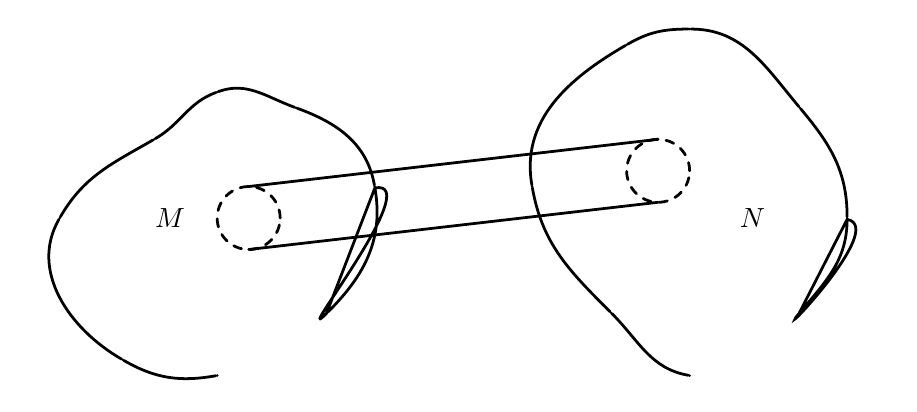
\begin{tikzpicture}[%
    scale=2,
    line width=1pt,
    line cap=round,
]
    \begin{scope}[%
        every node/.style={
            fill=black,
            circle,
            inner sep=0pt,
            outer sep=0pt
        }
    ]
        \node at (0,0) (a) {};
        \node at (-0.6,0.1) (b) {};
        \node at (-1,1) (c) {};
        \node at (-0.4,1.5) (d) {};
        \node at (0, 1.8) (e) {};
        \node at (0.5, 1.7) (f) {};
        \node at (1,1.2) (g) {};
        \node at (0.7,0.4) (h) {};
        \node at (3,0) (a1) {};
        \node at (2.5,0.4) (b1) {};
        \node at (2,1.2) (c1) {};
        \node at (2.6,2.1) (d1) {};
        \node at (3, 2.2) (e1) {};
        \node at (3.7, 1.7) (f1) {};
        \node at (4,1) (g1) {};
        \node at (3.7,0.4) (h1) {};
    \end{scope}
    \node at (-0.3,1) (i) {$M$};
    \node at (3.4,1) (i1) {$N$};
    \draw (a) to [out=-170,in=-30] (b)
              to [out=150,in=-120] (c)
              to [out=60,in=-150] (d)
              to [out=30,in=-160] (e)
              to [out=20,in=160] (f)
              to [out=-20,in=100] (g)
              to [out=-80,in=45] (h)
              to [out=-135,in=10] cycle;
    \draw (a1) to [out=170,in=-45] (b1)
               to [out=135,in=-80] (c1)
               to [out=100,in=-150] (d1)
               to [out=30,in=180] (e1)
               to [out=0,in=130] (f1)
               to [out=-50,in=90] (g1)
               to [out=-90,in=50] (h1)
               to [out=-130,in=-10] cycle;
    \draw[dashed] (0.2,1) circle (0.2);
    \draw[dashed] (2.8,1.3) circle (0.2);
    \draw (0.2,1.2) -- (2.8,1.5);
    \draw (0.2,0.8) -- (2.8,1.1);
\end{tikzpicture}
                \caption{Example of a Zero Surgery.}
                \label{fig:surgery_theory_a_zero_surgery}
            \end{figure}
            Let $\mathcal{M}^{n}$ be an $n$ dimensional manifold.
            Embed
            $S^{k}\times D^{n-k}$ into $\mathcal{M}^{n}$.
            Let $\partial(X)$ be the boundary of $X$.
            Then we have:
            \begin{align*}
                \partial(S^{k}\times {D^{n-k}})
                &=S^{k}\times{S^{n-k-1}}
                &
                \dim(S^{k+1}\times{D^{n-k-1})}
                &=\dim(S^{k}\times{D^{n-k}})=n
            \end{align*}
            Remove $\partial(S^{k}\times{D^{n-k}})$ and glue on
            $S^{k+1}\times{D}^{n-k-1}$. We alse have that
            $\partial(D^{k+1}\times{S^{n-k-1}})=S^{k}\times{S^{n-k-1}}$.
            Glue $\mathcal{M}^{n}\cup(D^{k+1}\times S^{n-k-1})$
            along $\partial(S^{k}\times{S^{n-k-1}})$.
            \begin{figure}[H]
                \centering
                \captionsetup{type=figure}
                \begin{tikzpicture}[%
    font=\scriptsize,
    scale=1.3,
    line width=1pt,
    line cap=round,
    >={Latex[black]},
    every edge/.style={draw=black,very thick}
]
    \draw[densely dashed] (0,0) circle (1.1);
    \draw[thick] (0,0) circle (2.5);
    \node at (0,2) {$\mathcal{M}$};
    \node at (0,0) {$S^{k}\times D^{n-k}$};
    \node at (0,-1.4)
        {
            $\partial\big(S^{k}\times{D^{n-k}}\big)%
             =S^{k}\times{S^{n-k-1}}$
        };
    \begin{scope}[%
        every node/.style={
            fill=black,
            circle,
            inner sep=0pt,
            outer sep=0pt
        }
    ]
        \node at (5,0) (a) {};
        \node at (4.4,0.1) (b) {};
        \node at (4,1) (c) {};
        \node at (4.6,1.5) (d) {};
        \node at (5, 1.8) (e) {};
        \node at (5.5, 1.7) (f) {};
        \node at (6,1.2) (g) {};
        \node at (5.7,0.4) (h) {};
    \end{scope}
    \node at (5,0.8) {$D^{k+1}\times{S^{n-k}}$};
    \draw[>=latex,->] (3.6,0.7)--(1.4,0.2);
    \node at (4.8,-0.5) {Glue Along Boundary};
    \draw (a) to [out=-170,in=-30] (b)
              to [out=150,in=-110] (c)
              to [out=70,in=-140] (d)
              to [out=40,in=-160] (e)
              to [out=20,in=150] (f)
              to [out=-30,in=100] (g)
              to [out=-80,in=45] (h)
              to [out=-135,in=10] cycle;
\end{tikzpicture}
                \caption[More Complicated Surgery Example.]
                        {Gluing $D^{k+1}\times S^{n-k}$ along
                         $\partial(S^{k}\times D^{n-k})$. The new manifold is
                         $\mathcal{M}^{n}\setminus(S^{k}\times%
                          D^{n-k}\coprod(D^{k+1}\times S^{n-k-1})$}
                \label{fig:surgery_theory_glueing_S_k_D_n_k_to_M}
            \end{figure}
            We now consider $k$ surgeries
            $\mathcal{M}\overset{\textrm{k-surgery}}%
                                {\longrightarrow}\mathcal{N}$.
            We have seen
            $S^{2}\overset{\textrm{0-surgery}}{\longrightarrow}T^{2}$.
            Note: $\pi_{1}(S^{2})$ is trivial, and
            $\pi_{1}(T^{2})=\mathbb{Z}^{2}$. This happens because $n<5$. When
            $n\geq{5}$, we have the following result.
            \begin{theorem}
                If $\mathcal{M}$ is an $n$ dimensional manifold, $n\geq{5}$,
                and if $\mathcal{N}$ is the result of a $k$ surgery on
                $\mathcal{M}$, then $\pi_{1}(\mathcal{M})=\pi_{1}(\mathcal{N})$.
            \end{theorem}
        \subsubsection{More On Surgery Exact Sequences}
            Recall that a surgery exact sequence looks like the following:
            \begin{equation*}
                \underset{\textrm{Group}}
                {\underbrace{L_{n+1}(\mathbb{Z}\pi_{1}\mathcal{M})}}
                \rightarrow\cdots\rightarrow
                \underset{\textrm{Not a Group}}
                {\underbrace{S^{Cat}(\mathcal{M}^{n})}}
                \rightarrow
                \underset{\textrm{Group}}
                {\underbrace{[M,G/0]}}
                \rightarrow \underset{\textrm{Group}}
                {\underbrace{L_{n}(\mathbb{Z}\pi_{1}(\mathcal{M}))}} 
            \end{equation*}
            An exact sequence of groups is of then form
            $G_{n+1}\overset{g_{n}}{\rightarrow}%
             G_{n}\rightarrow \hdots$,
            where $\Ima(g_n)=\ker(g_{n-1})$. We refine our notion of a
            surgery exact sequence:
            \begin{equation*}
                \cdots\rightarrow
                L_{n+1}(\mathbb{Z}\pi_{1}(\mathcal{M}))
                \dashrightarrow{S^{Cat}}(\mathcal{M})
                \overset{g}{\rightarrow}[M,G/o]
                \overset{\sigma}{\rightarrow}
                L_{n}(\mathbb{Z}\pi_{1}(\mathcal{M}))
            \end{equation*}
            The dotted line means
            $L_{n+1}(\mathbb{Z}\pi_{1}(\mathcal{M}))$
            acts on $S^{Cat}(\mathcal{M})$. Exact means $\Ima(g)=\ker(\sigma)$.
            Each element $f\in{[M,G/o]}$ either pulls back to $\emptyset$ or
            something non-empty. If the pullback is non-empty, you get a blob
            in $S^{Cat}(\mathcal{M})$: $f^{-1}(\{x\})$. But:
            \begin{equation}
                \bigcup_{f\in[M,G/o]}g^{-1}(\{f\})=S^{Cat}(\mathcal{M})
            \end{equation}
            This process creates a partition of $S^{Cat}(\mathcal{M})$. Now,
            $L_{n+1}(\mathbb{Z}(\pi_{1}\mathcal{M}))$ acts on
            $S^{Cat}(\mathcal{M})$ in some fashion. Partition the space into
            orbits. Exactness here means that partitioning by point inverses
            is the same as partitioning by orbits. That is, the two partitions
            are identical. See Fig.~\ref{fig:surgery_theory_partition_of_S_Cat}
            for a partitioning into orbits.
            \newpage
            \begin{figure}[H]
                \centering
                \captionsetup{type=figure}
                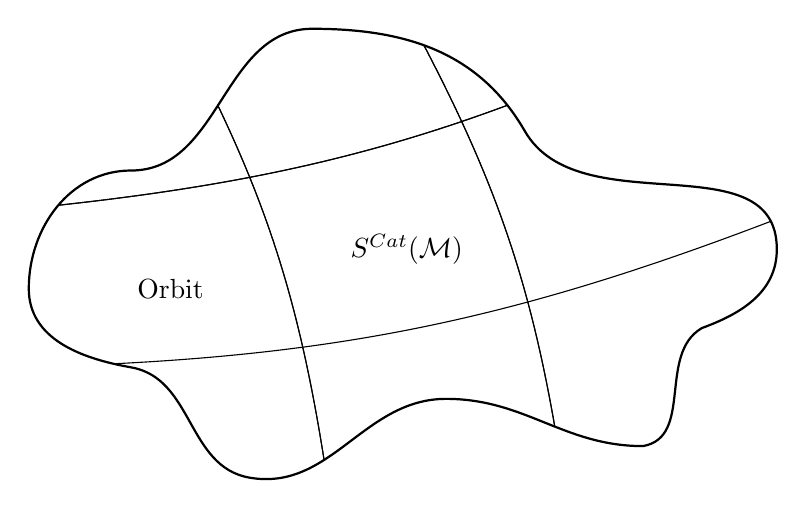
\begin{tikzpicture}
    \draw[line width=0.8pt]
        (0.2,2.5) to[out=-90,in=170]
        (1.5,1.5) to[out=-10,in=170]
        (3,0.1) to[out=-10,in=180]
        (5.5,1.1) to[out=0,in=180]
        (8,0.5) to[out=10,in=-150]
        (8.75,2) to[out=20,in=-90]
        (9.7,3) to[out=90,in=-60]
        (6.5,4.5) to[out=120,in=0]
        (3.8,5.8) to[out=180,in=0]
        (1.5,4) to[out=180,in=90] cycle;
    \clip (0.2,2.5) to[out=-90,in=170] (1.5,1.5)
                    to[out=-10,in=170] (3,0.1)
                    to[out=-10,in=180] (5.5,1.1)
                    to[out=0,in=180] (8,0.5)
                    to[out=10,in=-150] (8.75,2)
                    to[out=20,in=-90] (9.7,3)
                    to[out=90,in=-60] (6.5,4.5)
                    to[out=120,in=0] (3.8,5.8)
                    to[out=180,in=0] (1.5,4)
                    to[out=180,in=90] cycle;
    \draw (4,0) to[bend right=10] (2,6) to (5,6)
                to [bend left=10] (7,0) to cycle;
    \draw (7,0) to[bend right=10] (5,6) to (10,6)
                to (10,0) to cycle;
    \draw (0,1.5) to (0,3.5) to [bend right=10] (9,6)
                  to (10,6) to (10,3.5) to [bend left=10] cycle;
    \draw (0,0) to (4,0) to[bend right=10] (2,6)
                to (0,6) to (0,0) to cycle;
    \draw (0,6) to (0,3.5) to[bend right=10] (9,6)
                to (0,6) to cycle;
    \node at (2,2.5) {Orbit};  
    \node at (5,3) {$S^{Cat}(\mathcal{M})$};
\end{tikzpicture}
                \caption{Partition of $S^{Cat}(\mathcal{M})$.}
                \label{fig:surgery_theory_partition_of_S_Cat}
            \end{figure}
            The next object to talk about is
            $L_{n}(\mathbb{Z}\pi_{1}(\mathcal{M}))$.
            These are called Wall groups. They are difficult to compute,
            but there are some facts that are known about them:
            \begin{itemize}
                \item Wall groups only have 2-torsion.
                \begin{itemize}
                    \item 2-torsion means that elements
                          of finite order have order $2$.
                    \item This implies the groups are Abelian.
                \end{itemize}
                \item They can be orientable or not.
                \begin{itemize}
                    \item $L_{n}(\mathbb{Z}\pi_{1}(\mathcal{M})^{\pm})$
                           indicates orientable or not.
                \end{itemize}
            \end{itemize}
    \subsection{Lecture 3: Vector Bundles}
        \subsubsection{Group Rings}
            \begin{definition}
                If $G$ is a group and $R$ is a ring, then the group ring $RG$
                is the collection of all finite linear combinations
                (Formal Sums): $r_{1}g_{1}+\hdots+r_{n}g_{n}$, where
                $r_{k}\in{R}$ and $g_{k}\in{G}$.
            \end{definition}
            \begin{example}
                If $G$ is a group, and
                $\mathbb{Z}G=\{\sum_{k=0}^{n}n_{k}g_{k}:%
                 n_{k}\in\mathbb{Z},g_{k}\in{G}\}$, then $\mathbb{Z}G$ is a
                group ring. This is a special group ring, denoted
                $\textrm{SP}_{\mathbb{Z}}(G)$.
            \end{example}
            \begin{theorem}
                If $R$ is a ring and $G$ is a group, then
                the group ring $RG$ is a ring.
            \end{theorem}
            From the previous lecture we saw that
            $L_{n+1}(\mathbb{Z}\pi_{1}(\mathcal{M}))$ is a group. But from the
            previous theorem, we have that $\mathbb{Z}\pi_{1}(\mathcal{M})$ is
            a ring. So, we may thing of the $L_{n}$ as a \textit{Functor}:
            $L_{n}:\textrm{Rings}\rightarrow\textrm{Groups}$.
            To recap the notation, $S(\mathcal{M})$ is the Surgery Structure
            Set on the manifold $\mathcal{M}$, and
            $L_{n}(\mathbb{Z}\pi_{1}(\mathcal{M}))$ is a Wall Group.
        \subsubsection{Matrices and Vector Bundles}
            The next monster we need to understand in the
            Surgery Exact Sequence is the
            $[\mathcal{M},G/o]$ that keep appearing.
            First, a quick recap on some notions in
            linear algebra.
            \begin{definition}
                An orthogonal matrix is an invertible
                square matrix $A$ such that
                $A^{T}=A^{-1}$
            \end{definition}
            Let $\mathcal{O}(n)$ be the group of $n\times{n}$ orthogonal
            matrices. There is a simple map then from
            $\mathcal{O}(n)$ to $\mathcal{O}(n+1)$,
            $\psi_{n}:\mathcal{O}(n)\rightarrow\mathcal{O}(n+1)$,
            defined by:
            \begin{equation*}
                \psi_{n}(A)=
                \left[%
                    \begin{array}{c|c}
                        A&0\\
                        \hline
                        0&1
                    \end{array}
                \right]
            \end{equation*}
            We can also define a map
            $\varphi_{nm}:%
             \mathcal{O}(n)\times\mathcal{O}(m)%
             \rightarrow\mathcal{O}(n+m)$ defined
            by:
            \begin{equation*}
                \varphi_{nm}(A,B)=
                \left[%
                    \begin{array}{c|c}
                        A&0\\
                        \hline
                        0&B
                    \end{array}
                \right]
            \end{equation*}
            This is, in general, not a bijection.
            From this we can create a sequence:
            \begin{equation*}
                \mathcal{O}(1)
                \overset{\psi_{1}}{\longrightarrow}\mathcal{O}(2)
                \overset{\psi_{2}}{\longrightarrow}\mathcal{O}(3)
                \overset{\psi_{3}}{\longrightarrow}\mathcal{O}(4)
                \overset{\psi_{4}}{\longrightarrow}\cdots
                \mathcal{O}(n)\overset{\psi_{n}}{\longrightarrow}\cdots
            \end{equation*}
            We can then define $\mathcal{O}$ as the
            \textit{Direct Limit} of this sequence:
            \begin{equation*}
                \mathcal{O}=\underset{n\rightarrow\infty}{\lim}\mathcal{O}(n)
            \end{equation*}
            Now, let $\mathcal{M}$ be a manifold. An $n$ dimensional vector
            bundle is a map $P:E\rightarrow\mathcal{M}$ such that, for each
            point $x\in\mathcal{M}$, the \textit{fiber} of $x$, the pre-image
            $p^{-1}(x)$, is homeomorphic to $\mathbb{R}^{n}$.
            \begin{definition}
                The fiber of a point $y$ in a set $Y$ under the map
                $f:X\rightarrow{Y}$ is the pre-image $f^{-1}(y)\subset{X}$.
            \end{definition}
            \begin{definition}
                A real $n$ dimensional vector bundle on a manifold $\mathcal{M}$
                is a manifold $E$ and a continuous map
                $p:E\rightarrow\mathcal{M}$ such that, for all
                $x\in\mathcal{M}$, the fiber of $x$ is homeomorphic to
                $\mathbb{R}^{n}$ and there exists an open set $\mathcal{U}$
                such that $x\in\mathcal{U}$ and $p^{-1}(\mathcal{U})$ is
                homeomorphic to $\mathcal{U}\times\mathbb{R}^{n}$
            \end{definition}
            The requirement that there is an open neighborhood $\mathcal{U}_{x}$
            for all $x$ such that $p^{-1}(\mathcal{U})$ is homeomoprhic to
            $\mathcal{U}_{x}\times\mathbb{R}^{n}$ is called
            \textit{local triviality}. There is another notion called
            \textit{global triviality}.
            \begin{example}
                A classic example is a cylinder with a disk (Or the boundary of
                a cylinder with the circle). Given a point $(x,y,z)$ in the
                cylinder, collapse this (Or project it) down onto the $xy$
                plane by the map $p(x,y,z)=(x,y)$. This is continuous, and is
                an example of a vector bundle:
                $(D^{1},D^{1}\times\mathbb{R},p)$. The pre-image, or fiber, of
                any point in $D^{1}$ is a line, which is certainly homeomorphic
                to $\mathbb{R}$. Again, taking any point $x$ and looking at an
                open ball about that point that is entirely contained within
                $D^{1}$, the pre-image $p^{-1}(B_{r}(x))$ is another cylinder,
                which is homeomorphic to $\mathbb{R}^{3}$, which is itself
                homeomorphic to $B_{r}(x)\times\mathbb{R}^{1}$. The fibers of
                $x$ and $\mathcal{U}$ are shown in
                Fig.~\ref{fig:Simple_Vector_Bundle_Cylinder_to_Disk}
            \end{example}
            \begin{figure}[H]
                \centering
                \captionsetup{type=figure}
                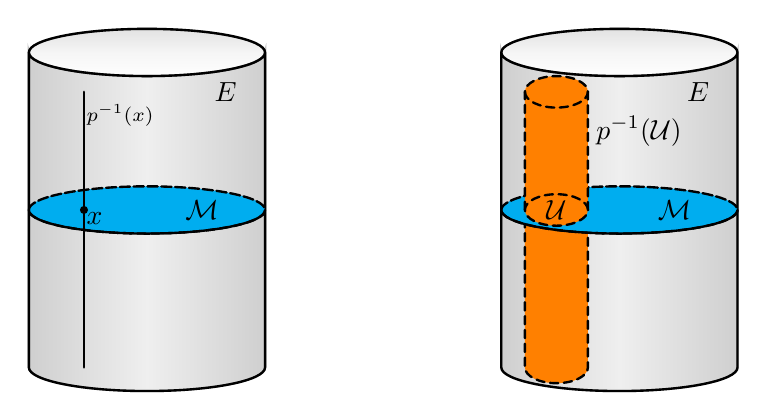
\begin{tikzpicture}[%
    line width=0.3mm,
    line cap=round,
]
    \draw[%
        left color=gray!50!black,
        right color=gray!50!black,
        middle color=gray!50,
        shading=axis,
        opacity=0.25
    ]   (1.5,0) to (1.5,4) arc (360:180:1.5cm and 0.3cm)
                to (-1.5,0) arc (180:360:1.5cm and 0.3cm);
    \draw[%
        top color=gray!90!,
        bottom color=gray!2,
        middle color=gray!30,
        shading=axis,
        opacity=0.25
    ]   (0,4) circle (1.5cm and 0.3cm);
    \draw (-1.5,4) to (-1.5,0) arc (180:360:1.5cm and 0.3cm)
                   to (1.5,4) (0,4) circle (1.5cm and 0.3cm);
    \draw[fill=cyan,densely dashed]
        (-1.5,2) arc (180:0:1.5cm and 0.3cm) 
                 arc (360:0:1.5cm and 0.3cm);
    \draw (-1.5,2) arc (180:360:1.5cm and 0.3cm);
    \node[%
        circle,
        fill=black,
        draw=black,
        inner sep=0pt,
        minimum size=2pt
    ]   at (-0.8,2) {};
    \node at (-0.9,2.1) [below right] {$x$};
    \node at (0.7,2) {$\mathcal{M}$};
    \node at (1,3.5) {$E$};
    \node at (-0.9,3.2) [right] {\scriptsize{$p^{-1}(x)$}};
    \draw (-0.8,0) to (-0.8,3.5);
    % Shift for the second cylinder.
    \begin{scope}[xshift=6cm]
        \draw[%
            left color=gray!50!black,
            right color=gray!50!black,
            middle color=gray!50,
            shading=axis,
            opacity=0.25
        ]   (1.5,0) to (1.5,4) arc (360:180:1.5cm and 0.3cm)
                    to (-1.5,0) arc (180:360:1.5cm and 0.3cm);
        \draw[%
            top color=gray!90!,
            bottom color=gray!2,
            middle color=gray!30,
            shading=axis,
            opacity=0.25
        ]   (0,4) circle (1.5cm and 0.3cm);
        \draw (-1.5,4) to (-1.5,0) arc (180:360:1.5cm and 0.3cm)
                       to (1.5,4) (0,4) circle (1.5cm and 0.3cm);
        \draw[densely dashed, fill=orange]
            (-0.4,2) to (-0.4,0) arc (360:180:4mm and 2mm)
                     to (-1.2,2);
        \draw[fill=cyan,densely dashed]
            (-1.5,2) arc (180:0:1.5cm and 0.3cm) 
                     arc (360:0:1.5cm and 0.3cm);
        \draw (-1.5,2) arc (180:360:1.5cm and 0.3cm);
        \draw[densely dashed, fill=orange]
            (-1.2,2) to (-1.2,3.5) arc (180:0:4mm and 2mm)
                     to (-0.4,2);
        \draw[densely dashed,fill=orange]
            (-0.8,2) circle (4mm and 2mm);
        \draw[densely dashed]
            (-1.2,3.5) arc (180:360:4mm and 2mm);
        \node at (-0.8,2) {$\mathcal{U}$};
        \node at (0.7,2) {$\mathcal{M}$};
        \node at (1,3.5) {$E$};
        \node at (0.25,3) {$p^{-1}(\mathcal{U})$};
    \end{scope}
\end{tikzpicture}
                \caption{Example of a Vector Bundle:
                         $(D^{1},D^{1}\times\mathbb{R},p)$.}
                \label{fig:Simple_Vector_Bundle_Cylinder_to_Disk}
            \end{figure}
            \begin{example}
                If $\mathcal{M}$ is a manifold,
                $E=\mathcal{M}\times\mathbb{R}^{n}$, and if
                $p:E\rightarrow\mathcal{M}$ is defined by $p(x,\mathbf{y})=x$
                for all $(x,\mathbf{y})\in\mathcal{M}\times\mathbb{R}^{n}$,
                then $(E,\mathcal{M},p)$ is a vector bundle. This is called
                the trivial $n$ dimensional vector bundle of $\mathbb{R}^{n}$.
                The fibers of points $x\in\mathcal{M}$ are $\mathbb{R}^{n}$,
                which is homeomorphic to $\mathbb{R}^{n}$. Given any open set
                $\mathcal{U}$ containing $x$, the pre-image is
                $\mathcal{U}\times\mathbb{R}^{n}$.
            \end{example}
            \begin{example}
                The M\"{o}bius strip can be seen as a vector bundle
                $S^{1}\times[0,1]\rightarrow[0,1]$ where the map
                $(x,t)\rightarrow{x}$ is by a ``twist.'' This is a
                non-oreientable bundle which is non-trivial. It has local
                triviality, but no global triviality.
            \end{example}
            \begin{figure}[H]
                \centering
                \captionsetup{type=figure}
                \documentclass[crop,class=article]{standalone}
%----------------------------Preamble-------------------------------%
\usepackage{pgfplots, tikz}             % Drawing/graphing tools.
\pgfplotsset{compat=1.9}                % Version of pgfplots.
%--------------------------Main Document----------------------------%
\begin{document}
    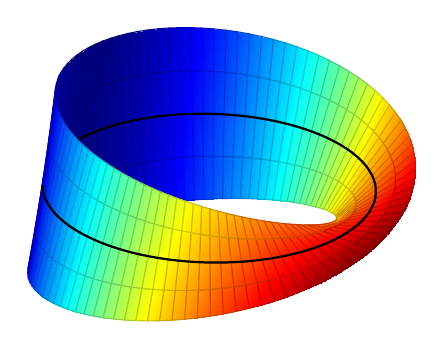
\begin{tikzpicture}
        \begin{axis}[
            hide axis,
            view={40}{40}
        ]
            \addplot3[%
                surf,
                shader=faceted interp,
                point meta=x,
                colormap/jet,
                samples=100,
                samples y=5,
                domain=0:360,
                y domain=-0.5:0.5
            ]   ({(1+0.5*y*cos(x/2)))*cos(x)},
                 {(1+0.5*y*cos(x/2)))*sin(x)},
                 {0.5*y*sin(x/2)});

            \addplot3[%
                samples=100,
                domain=-140:180,
                samples y=0,
                thick,
                line cap=round
            ]   ({cos(x)},{sin(x)},{0});
        \end{axis}
    \end{tikzpicture}
\end{document}
                \caption{M\"{o}bius Strip.}
                \label{fig:Surgery_Theory_Mobius_Strip_Vector_Bundle}
            \end{figure}
            Returning to our discussion of orthogonal matrices,
            $\mathcal{O}(n)$ is a group under matrix multiplication.
            The matrix $I_{n}$ is orthogonal, and if $A$ is orthogonal,
            then $(A^{-1})^{T}=(A^{T})^{T}=A$. But $(A^{-1})^{-1}=A$,
            and thus $A^{-1}$ is orthogonal as well. Thus we have
            an identity, associativity, and closure of inverses.
            Therefore $\mathcal{O}(n)$ is a group. This group can
            act on the set of $n$ dimensional vectors in
            $\mathbb{R}^{n}$ by the map
            $(A,\mathbf{v})\rightarrow{A\mathbf{v}}$,
            for all $A\in\mathcal{O}(n),\mathbf{v}\in\mathbb{R}^{n}$.
            Thus, we have the $\mathcal{O}(n)$ acts over the fibers
            of an $n$ dimensional real vector bundle
            $(E,\mathcal{M},p)$. $\mathcal{O}(1)$ is the identity.
            That is, the ``Do nothing,'' action on a 1 dimensional
            vector bundle. $\mathcal{O}(2)$ can perform
            \textit{reflections} and \textit{rotations} on the
            fibers. Endowed with this action, any real
            vector bundle of dimension $n$ is an example of
            a \textit{principal $\mathcal{O}(n)$ bundle}.
            If $g\in\mathcal{O}(n)$ and $v\in{E}$,
            then $p(gv)=g(p(v)$.
        \subsubsection{Principal G-Bundles}
            If $G$ is a group, and if $X$ is a
            topogolical space, then there is a
            structure/notion of a
            \textit{principal G-Bundle} on $X$.
            That is, $X$ has some bundle over it
            (The space $E$ from our previous discussion),
            and $G$ acts on the fibers of $X$. This is
            denoted $\Prin_{G}(X)$.
            \par\hfill\par
            Construction by John Milnor, Classifying space.
            No idea why I wrote this...
            \par\hfill\par
            If $G$ is a group, there is a complex (space) $BG$
            such that we may form the set:
            \begin{equation*}
                [\mathcal{M},BG]
                =\{f:\mathcal{M}\rightarrow{BG}\}/Homotopy
            \end{equation*}
            That is, the set of continuous maps from $\mathcal{M}$ to
            $BG$ modded out by homotopy. Two maps are equivalent if they
            are homotopic.
            \begin{theorem}
                There is a continuous surjective function
                $f:\Prin_{G}(\mathcal{M})\rightarrow%
                 [\mathcal{M},BG]$.
            \end{theorem}
            Elaborating more on the $BG$,
            $B$ is a \textit{functor}
            $B:\textrm{Groups}\rightarrow\textrm{Spaces}$.
            If $G$ is a finitely presented group,
            then $\pi_{1}(BG)=G$, and more over,
            for all $n\geq{2}$,
            $\pi_{n}(BG)=0$. That is, $\pi_{n}(BG)$
            is the trivial group for all $n\geq{2}$.
            $\pi_{1}(X)$ ca be seen as the
            \textit{homotopy class} of $[S^{1},X]$.
            $\pi_{n}$ the homotopy class for
            $[S^{n},X]$.
            \begin{example}
                $\pi_{1}(B\mathbb{Z})=\mathbb{Z}$.
                For all $n\geq{2}$,
                $\pi_{n}(B\mathbb{Z})=0$.
                Thus $B\mathbb{Z}$ is homotopy
                equivalent to $S^{1}$.
            \end{example}
        \subsubsection{Covering Spaces}
            \begin{definition}
                A covering space of a topological space $X$ is a space $E$ such
                that there exists a continuous surjection $p:E\rightarrow{X}$
                such that for all $x\in{X}$, there is an open set $\mathcal{U}$
                such that $x\in\mathcal{U}$ such that there exists a set of
                disjoint open sets $E_{r}\subset{E}$ where
                $p^{-1}(\mathcal{U})=\cup_{r}E_{r}$ and for all $r$, $p$ is a
                homeomorphism between $E_{r}$ and $\mathcal{U}$.
            \end{definition}
            \begin{example}
                The first example is $S^{1}$ and $\mathbb{R}$. Define the map
                $p:\mathbb{R}\rightarrow{S^{1}}$ by $p(x)=\exp(2\pi{i}x)$. This
                ``wraps,'' the real line around the circle over and over again.
                Given a point $y\in{S^{1}}$, the pre-image, or fiber, of $y$
                with respect to $p$ is $\{x+n:n\in\mathbb{Z}\}$ for some
                $x\in[0,1)$. Given a small enough neighborhood around $y$, the
                pre-image is of the form
                $\{x+n-\varepsilon,x+n+\varepsilon:n\in\mathbb{Z}\}$,
                which is a bunch of copies of $(0,1)$, or a bunch
                of copies of the neighborhood around $y$.
            \end{example}
            \begin{figure}[H]
                \centering
                \captionsetup{type=figure}
                \begin{tikzpicture}[>=Latex,line width=0.3mm,font=\scriptsize]
    \draw[<->] (-4,0) to (4,0);
    \draw (0,-2) circle (1);
    \begin{scope}[(-),draw=blue]
        \draw (0.5,-1.13397) arc (60:120:1);
        \draw (-0.5,0) to (0.5,0);
        \draw (-2.5,0) to (-1.5,0);
        \draw (2.5,0) to (1.5,0);
    \end{scope}
    \begin{scope}[%
        every node/.style={
            circle,
            fill=black,
            draw=black,
            inner sep=0pt,
            minimum size=2pt
        }
    ]
        \node at (0,-1) {};
        \node at (0,0) {};
        \node at (-2,0) {};
        \node at (2,0) {};
    \end{scope}
    \draw[->]  (-2,-0.2) to [out=-90,in=150] (-0.5,-0.8);
    \draw[->]  (2,-0.2) to [out=-90,in=30] (0.5,-0.8);
    \draw[->] (0,-0.2) to (0,-0.8);
    \node at (-0.6,-0.35) {$p$};
    \node at (0.15,-1.2) {$y$};
    \node at (0,0) [above] {$x$};
    \node at (2,0) [above] {$x+1$};
    \node at (-2,0) [above] {$x-1$};
    \node at (4,0) [above] {$\mathbb{R}$};
    \node at (1,-1) {$S^{1}$};
\end{tikzpicture}
                \caption{$\mathbb{R}$ is the Universal Cover of $S^{1}$.}
                \label{fig:Reals_Cover_Circle}
            \end{figure}
            \begin{definition}
                A universal covering space of a topological space $X$
                is a covering space $E$ of $X$ such that
                $E$ is simply connected.
            \end{definition}
            That is, if $E$ is a covering space of $X$, then we say
            that $E$ is a universal covering space if
            $\pi_{1}(E)=0$. In the previous example we saw that
            $\mathbb{R}$ is a covering space of $S^{1}$. But
            $\mathbb{R}$ is simply connected. That is,
            $\pi_{1}(\mathbb{R})=0$. Therefore $\mathbb{R}$ is a
            universal covering space of $S^{1}$. Up to homotopy equivalence,
            $B\mathbb{Z}^{n}=T^{n}$, the $n$ torus. This is because
            $\pi_{1}(B\mathbb{Z}^{n})=\mathbb{Z}^{n}$, and
            $\pi_{n}(B\mathbb{Z}^{n})=0$ for $n\geq{2}$.
            For $S^{n}$, if $n\geq{2}$ then $S^{n}$ is simply connected,
            $\pi_{1}(S^{n})=0$. But then the identity map makes
            $S^{n}$ a covering space for itself. That is,
            $id_{S^{n}}$ is a covering map. But since $S^{n}$ is
            simply connected ($n\geq{2}$), we have that
            $S^{n}$ is a universal covering of itself.
            Moreover, it can be shown that
            $S^{n}$ is a universal covering space of
            $\mathbb{R}P^{n}$ for $n\geq{2}$.
            All universal covering spaces are homotopy
            equivalent to each other.
        \subsubsection{Eilenburg-MacLane Spaces}
            \begin{definition}
                An Eilenberg-MacLane space is a topological space
                $X$ such that there exists a non-trivial group
                $G$ and an $n\in\mathbb{N}$ such that
                $\pi_{n}(X)=G$ and, for all $m\ne{n}$,
                $\pi_{m}(X)=0$.
            \end{definition}
            This $B$ functor takes a group $G$ and spits out
            an Eilenberg-MacLane space. That is,
            $\pi_{1}(BG)=G$, and $\pi_{n}(BG)=0$ for all
            $n\geq{2}$. Eilenberg-MacLane spaces are analogous to
            prime numbers in Number Theory, but for the
            study of topological spaces. These have a
            special notation:
            \begin{fnotation}{}{}
                An Eilenberg-MacLane space $X$ is of the type
                $K(G,n)$ if $\pi_{n}(X)=G$ and, for all
                $m\ne{n}$, $\pi_{m}(X)=0$. We write
                $X\in{K(G,n)}$.
            \end{fnotation}
            Every principal $G$ bundle over $\mathcal{M}$
            can be imagined as $[\mathcal{M},BG]$.
            A principal $\mathcal{O}(n)$ bundle can be
            identitifed with a map
            $f:\mathcal{M}\rightarrow{B}\mathcal{O}(n)$.
            For example, $f$ be the constant map.
            Constant maps are homotopic to each other. This
            is the easiest bundle.
    \subsection{Lecture 4: Principal G-Bundles}
        A brief discussion on complexes. A simplex
        is a generalization of the notation of a triangle.
        A triangle can be considered as the
        convex-hull of $3$ non-coplanar points.
        This is called a $2$-simplex. A $0$-simplex
        is thus a point, and a $1$-simplex is a line.
        This can be generalized to higher dimensions.
        A $3$-simplex is a tetrahedron,
        and an $n$-simplex is an $n$ dimensional triangle,
        defined on $n+1$ non-hyper-coplanar points.
        \begin{figure}[H]
            \centering
            \captionsetup{type=figure}
            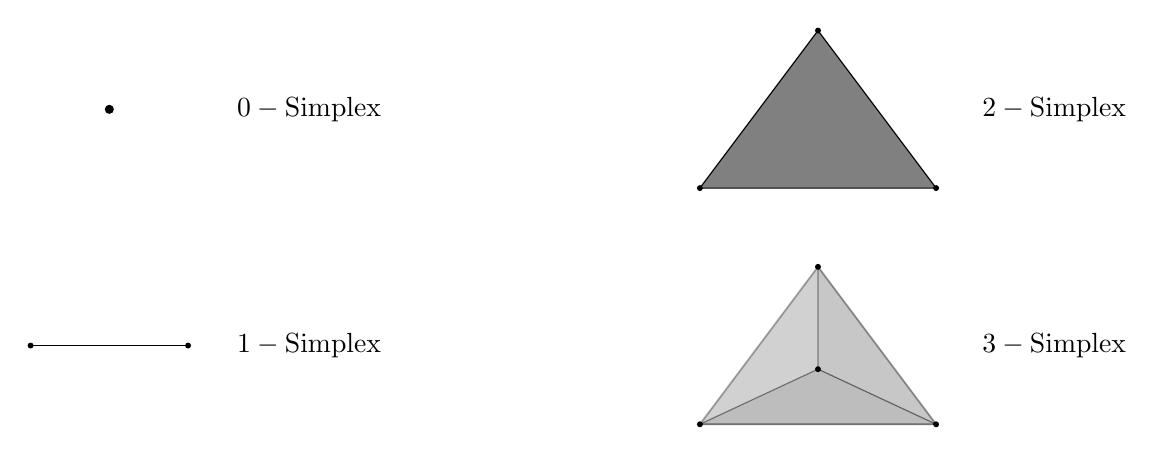
\begin{tikzpicture}
    \node at (1.5,1) [right] {$0-\textrm{Simplex}$};
    \node at (1.5,-2) [right] {$1-\textrm{Simplex}$};
    \node at (12,1) {$2-\textrm{Simplex}$};
    \node at (12,-2) {$3-\textrm{Simplex}$};
    \draw[fill=black] (0,1) circle (0.05);
    \draw[fill=black] (-1,-2) circle (0.03);
    \draw[fill=black] (1,-2) circle (0.03);
    \draw[draw=black] (1,-2) -- (-1,-2);
    \draw[fill=gray] (9,2)--(7.5,0)--(10.5,0)--cycle;
    \draw[fill=black] (9,2) circle (0.03);
    \draw[fill=black] (7.5,0) circle (0.03);
    \draw[fill=black] (10.5,0) circle (0.03);
    \draw[fill=gray,opacity=0.2]
        (9,-1)--(7.5,-3)--(9,-2.3)--cycle;
    \draw[fill=gray,opacity=0.3]
        (9,-1)--(10.5,-3)--(9,-2.3)--cycle;
    \draw[fill=gray,opacity=0.4]
        (9,-2.3)--(7.5,-3)--(10.5,-3)--cycle;
    \draw[fill=gray,opacity=0.2, thick]
        (9,-1)--(7.5,-3)--(10.5,-3)--cycle;
    \draw[fill=black] (9,-1) circle (0.03);
    \draw[fill=black] (7.5,-3) circle (0.03);
    \draw[fill=black] (10.5,-3) circle (0.03);
    \draw[fill=black] (9,-2.3) circle (0.03);
\end{tikzpicture}
            \caption{Examples of Simplices.}
            \label{fig:surgery_theory_simplexes}
        \end{figure}
        A simplicial complex is a set of simplices
        $\mathcal{H}$ such that the face of any element
        of $\mathcal{H}$ is also contained in $\mathcal{H}$,
        and the intersection of two simplices
        $\sigma_{1},\sigma_{2}\in \mathcal{K}$ is a
        face of both $\sigma_{1}$ and $\sigma_{2}$.
        We return to studying surgery exact sequences
        for $n\geq 5$. Let $\mathcal{M}$ be an $n$
        dimensional manifold, and let $G=\pi_{1}(\mathcal{M})$.
        In our surgery exact sequence we still have this
        mysterious object $[\mathcal{M},G/Cat]$. Let Cat
        be either PL or Top. The generalized Poincare
        Conjecture says that, for $n\geq 5$,
        $S^{PL}(S^{n})=S^{Top}(S^{n})=\{S^{n}\}$.
        Let $\mathcal{M}=S^{n}$. Then
        $G=\pi_{1}(\mathcal{M})=\{e\}$.
        Then we have the following:
        \begin{figure}[H]
            \centering
            \captionsetup{type=figure}
            \documentclass[crop,class=article]{standalone}
%----------------------------Preamble-------------------------------%
%---------------------------Packages----------------------------%
\usepackage{geometry}
\geometry{b5paper, margin=1.0in}
\usepackage[T1]{fontenc}
\usepackage{graphicx, float}            % Graphics/Images.
\usepackage{natbib}                     % For bibliographies.
\bibliographystyle{agsm}                % Bibliography style.
\usepackage[french, english]{babel}     % Language typesetting.
\usepackage[dvipsnames]{xcolor}         % Color names.
\usepackage{listings, lstlinebgrd}      % Verbatim-Like Tools.
\usepackage{mathtools, esint, mathrsfs} % amsmath and integrals.
\usepackage{amsthm, amsfonts}           % Fonts and theorems.
\usepackage{tabularx}
\usepackage{tcolorbox}                  % Frames around theorems.
\usepackage{upgreek}                    % Non-Italic Greek.
\usepackage{paracol}                    % Two-column styling.
\usepackage{wrapfig}                    % Wrap text around figure.
\usepackage{fmtcount, etoolbox}         % For the \book{} command.
\usepackage[newparttoc]{titlesec}       % Formatting chapter, etc.
\usepackage{titletoc}                   % Allows \book in toc.
\usepackage[nottoc]{tocbibind}          % Bibliography in toc.
\usepackage[titles]{tocloft}            % ToC formatting.
\usepackage{multicol, enumitem}         % Multi-column/enumerate.
\usepackage{import}                     % Import external files.
\usepackage{pgfplots, tikz}             % Drawing/graphing tools.
\usetikzlibrary{
    calc,                   % Calculating right angles and more.
    angles,                 % Drawing angles within triangles.
    arrows.meta,            % Latex and Stealth arrows.
    quotes,                 % Adding labels to angles.
    positioning,            % Relative positioning of nodes.
    decorations.markings,   % Adding arrows in the middle of a line.
    patterns,
    arrows,
    shapes,
    shapes.geometric,
    cd,
    hobby,
    babel
}                                       % Libraries for tikz.
\pgfplotsset{compat=1.9}                % Version of pgfplots.
\usepackage[font=scriptsize,
            labelformat=simple,
            labelsep=colon]{subcaption} % Subfigure captions.
\usepackage[font={scriptsize},
            hypcap=true,
            labelsep=colon]{caption}    % Figure captions.
\usepackage{hyperref}                   % Allows for hyperlinks.
\hypersetup{
    colorlinks=true,
    linkcolor=blue,
    filecolor=magenta,
    urlcolor=Cerulean,
    citecolor=SkyBlue
}                           % Colors for hyperref.
\usepackage[toc,acronym,nogroupskip]{glossaries} % Glossaries and acronyms.
\usepackage[subpreambles=false]{standalone}      % Complileable sub files.

% Various font stuff from kiwi.
% Use this for Times text and Computer Modern math
%\usepackage{times}

% Quite nice
%\usepackage[charter, greekfamily=, greekuppercase=italicized]{mathdesign}
%\usepackage[utopia, greekuppercase=italicized]{mathdesign}    % Math is narrower

% Use this for Times text and math
%\usepackage{newtxtext}
%\usepackage[libertine,cmintegrals]{newtxmath}
%\usepackage{fix-cm}

%\usepackage{txfontsb}
% or
%\usepackage{mathptmx}

%\usepackage[scaled=0.92]{helvet}
%\renewcommand{\rmdefault}{ptm}

%\usepackage{mathpazo}    % add possibly `sc` and `osf` options
%\usepackage{eulervm}

%\usepackage{fourier}
%\renewcommand{\rmdefault}{ptm}
%\usepackage{mathptm}

%\usepackage{fontspec}
%\setmainfont{lmodern}

%\usepackage[varg]{txfonts}
%\usepackage{fouriernc}
%\usepackage{mathpazo}

%\usepackage{bookman}
%\usepackage[scaled]{uarial}
%\usepackage[scaled]{helvet}
%\renewcommand*\familydefault{\sfdefault}
%\usepackage[math]{anttor}

%\newcommand\fgeorgia{\fontfamily{jvn}\selectfont}
%\newcommand\ftimes{\fontfamily{ptm}\selectfont}
%\newcommand\fhelvetica{\fontfamily{phv}\selectfont}
%\newcommand\fcourier{\fontfamily{pcr}\selectfont}
%\newcommand\fbookman{\fontfamily{pbk}\selectfont}
%\newcommand\fnewcentury{\fontfamily{pnc}\selectfont}
%\newcommand\fpalatino{\fontfamily{ppl}\selectfont}
%\newcommand\favantgarde{\fontfamily{pag}\selectfont}
%\newcommand\fnormal{\normalfont}
%\newcommand\fsize[1]{\ifnum#1>0\fontsize{#1}{#1}\selectfont\else\normalsize\fi}
%------------------------Theorem Styles-------------------------%
% Define theorem style for default spacing and normal font.
\newtheoremstyle{normal}
    {\topsep}               % Amount of space above the theorem.
    {\topsep}               % Amount of space below the theorem.
    {}                      % Font used for body of theorem.
    {}                      % Measure of space to indent.
    {\bfseries}             % Font of the header of the theorem.
    {}                      % Punctuation between head and body.
    {.5em}                  % Space after theorem head.
    {}

% Define theorem style for default spacing with italicized font.
\newtheoremstyle{normalit}{\topsep}{\topsep}
                {\itshape}{}{\bfseries}{}{.5em}{}

% Italic header environment.
\newtheoremstyle{thmit}{\topsep}{\topsep}{}{}{\itshape}{}{0.5em}{}

% Define italicized environments.
\theoremstyle{normalit}
\newtheorem{theorem}{Theorem}[section]
\newtheorem{lemma}{Lemma}[section]
\newtheorem{corollary}{Corollary}[section]
\newtheorem{proposition}{Proposition}[section]
\newtheorem*{theorem*}{Theorem}

% Define environments with italic headers.
\theoremstyle{thmit}
\newtheorem*{solution}{Solution}
\newtheorem*{fsolution}{Solution}

% Define default environments.
\theoremstyle{normal}
\newtheorem{example}{Example}[section]
\newtheorem{definition}{Definition}[section]
\newtheorem{problem}{Problem}[section]
\newtheorem{question}{Question}[section]
\newtheorem{remark}{Remark}[section]
\newtheorem{properties}{Properties}[section]
\newtheorem{notation}{Notation}[section]
\newtheorem{axiom}{Axiom}[section]
\newtheorem*{properties*}{Properties}
\newtheorem*{remark*}{Remark}
\newtheorem*{definition*}{Definition}
\theoremstyle{plain}

% Define framed environment.
\tcbuselibrary{most}
\newtcbtheorem[use counter*=theorem]{ftheorem}{Theorem}%
    {colback=green!5,colframe=green!35!black,
     fonttitle=\bfseries\upshape}{th}

\newtcbtheorem[use counter*=example]{fdefinition}{Definition}%
    {fonttitle=\bfseries\upshape,
     colback=blue!5!white,colframe=blue!75!black}{def}

\newtcbtheorem[use counter*=example]{fexample}{Example}%
    {fonttitle=\bfseries\upshape,
     colback=red!5!white,colframe=red!75!black}{ex}

\newtcbtheorem[use counter*=notation]{fnotation}{Notation}%
    {fonttitle=\bfseries\upshape,
     colback=SeaGreen!5!white,colframe=SeaGreen!75!black}{ex}

\newtcbtheorem[use counter*=corollary]{fcorollary}{Corollary}%
    {fonttitle=\bfseries\upshape,
     colback=Orchid!5!white,colframe=Orchid!75!black}{ex}

\newenvironment{bproof}{\textit{Proof.}}{\hfill$\square$}
\tcolorboxenvironment{bproof}{blanker,breakable,left=5mm,
                             before skip=10pt,after skip=10pt,
                             borderline west={1mm}{0pt}{red}}
\tcolorboxenvironment{fsolution}
    {enhanced jigsaw,colframe=cyan,interior hidden,breakable}

%--------------------Declared Math Operators--------------------%
\DeclareMathOperator{\Refl}{Refl}           % Reflection operator.
\DeclareMathOperator{\Span}{Span}           % Span of a set of vectors.
\DeclareMathOperator{\Card}{Card}           % Cardinality of set.
\DeclareMathOperator{\Ord}{Ord}             % Ordinal of ordered set.
\DeclareMathOperator{\Tr}{Tr}               % Trace of matrix.
\DeclareMathOperator{\adjoint}{adj}         % Adjoint of matrix.
\DeclareMathOperator{\rk}{rk}               % Rank of operator.
\DeclareMathOperator{\nul}{nul}             % Null space of operator.
\DeclareMathOperator{\sgn}{sgn}             % Sign of a number.
\DeclareMathOperator{\multideg}{mutlideg}   % Multi-Degree (Graphs).
\DeclareMathOperator{\GCD}{GCD}             % Greatest common denominator.
\DeclareMathOperator{\LM}{LM}               % Leading monomial
\DeclareMathOperator{\LC}{LC}               % Leading coefficient.
\DeclareMathOperator{\LT}{LT}               % Leading term.
\DeclareMathOperator{\LCM}{LCM}             % Least common multiple.
\DeclareMathOperator{\Mon}{Mon}             % Monomial.
\DeclareMathOperator{\Spec}{Spec}           % Spectrum.
\DeclareMathOperator{\proj}{proj}           % Projection.
\DeclareMathOperator{\comp}{comp}           % Component.
\DeclareMathOperator{\sinc}{sinc}           % Sinc function.
\DeclareMathOperator{\Ima}{Im}              % Image of operator.
\DeclareMathOperator{\Prin}{Prin}           % Principal value.
\DeclareMathOperator{\Mod}{mod}             % Modulus.
%------------------------New Commands---------------------------%
\DeclarePairedDelimiter\norm{\lVert}{\rVert}
\DeclarePairedDelimiter\ceil{\lceil}{\rceil}
\DeclarePairedDelimiter\floor{\lfloor}{\rfloor}
\newcommand*\diff{\mathop{}\!\mathrm{d}}
\newcommand*\Diff[1]{\mathop{}\!\mathrm{d^#1}}
\renewcommand{\mod}{\ \Mod}
\renewcommand*{\glstextformat}[1]{\textcolor{RoyalBlue}{#1}}
\renewcommand{\glsnamefont}[1]{\textbf{#1}}
\renewcommand\labelitemii{$\circ$}
\renewcommand\thesubfigure{\arabic{chapter}.\arabic{figure}}
\renewcommand\thesubfigure{%
    \arabic{chapter}.\arabic{figure}.\arabic{subfigure}}
\addto\captionsenglish{\renewcommand{\figurename}{Fig.}}
%------------------------Book Command---------------------------%
\makeatletter
\renewcommand\@pnumwidth{1cm}
\newcounter{book}
\renewcommand\thebook{\@Roman\c@book}
\newcommand\book{%
    \if@openright
        \cleardoublepage
    \else
        \clearpage
    \fi
    \thispagestyle{plain}%
    \if@twocolumn
        \onecolumn
        \@tempswatrue
    \else
        \@tempswafalse
    \fi
    \null\vfil
    \secdef\@book\@sbook
}
\def\@book[#1]#2{%
    \ifnum \c@secnumdepth >-3\relax
        \refstepcounter{book}%
        \addcontentsline{toc}{book}{
            \bookname\ \thebook:\hspace{1em}#1
        }
    \else
        \addcontentsline{toc}{book}{#1}%
    \fi
    \markboth{}{}%
    {\centering
     \interlinepenalty \@M
     \normalfont
     \ifnum \c@secnumdepth >-2\relax
       \huge\bfseries \bookname\nobreakspace\thebook
       \par
       \vskip 20\p@
     \fi
     \Huge \bfseries #2\par}%
    \@endbook}
\def\@sbook#1{%
    {\centering
     \interlinepenalty \@M
     \normalfont
     \Huge \bfseries #1\par}%
    \@endbook}
\def\@endbook{
    \vfil\newpage
        \if@twoside
            \if@openright
                \null
                \thispagestyle{empty}%
                \newpage
            \fi
        \fi
        \if@tempswa
            \twocolumn
        \fi
}
\newcommand*\l@book[2]{%
    \ifnum \c@tocdepth >-2\relax
        \addpenalty{-\@highpenalty}%
        \addvspace{2.25em \@plus\p@}%
        \setlength\@tempdima{3em}%
        \begingroup
            \parindent \z@ \rightskip \@pnumwidth
            \parfillskip -\@pnumwidth
            {
                \leavevmode
                \Large \bfseries #1\hfil \hb@xt@\@pnumwidth{
                    \hss #2
                }
            }
            \par
            \nobreak
            \global\@nobreaktrue
            \everypar{\global\@nobreakfalse\everypar{}}%
        \endgroup
    \fi}
\newcommand\bookname{Book}
\renewcommand{\thebook}{\texorpdfstring{\Numberstring{book}}{book}}
\providecommand*{\toclevel@book}{-2}
\makeatother
\titlecontents{chapter}[0pt]
    {\bfseries}
    {\chaptername\ \thecontentslabel:\quad}
    {}
    {\hfill\contentspage}
\titleformat{\part}[display]
    {\Large\bfseries}
    {\partname\nobreakspace\thepart}
    {0mm}
    {\Huge\bfseries}
    \titlecontents{part}[0pt]
    {\large\bfseries}
    {\partname\ \thecontentslabel: \quad}
    {}
    {\hfill\contentspage}
\newcommand{\MarkRightAngle}[4][.3cm]
    {\coordinate (tempa) at ($(#3)!#1!(#2)$);
     \coordinate (tempb) at ($(#3)!#1!(#4)$);
     \coordinate (tempc) at ($(tempa)!0.5!(tempb)$);%midpoint
     \draw (tempa) -- ($(#3)!2!(tempc)$) -- (tempb);}
%--------------------------LENGTHS------------------------------%
% Spacings for the Table of Contents.
\addtolength{\cftsecnumwidth}{1ex}
\addtolength{\cftsubsecindent}{1ex}
\addtolength{\cftsubsecnumwidth}{1ex}
\addtolength{\cftfignumwidth}{1ex}
\addtolength{\cfttabnumwidth}{1ex}

% Spacing for multi-column and enumerate environments.
\setlength{\multicolsep}{6pt}
\setlist[enumerate]{itemsep=0pt,topsep=3pt}

% Indent and paragraph spacing.
\setlength{\parindent}{0em}
\setlength{\parskip}{0em}
%--------------------------Main Document----------------------------%
\begin{document}
    \begin{tikzpicture}[>=latex,->,scale=1.4]
        \node (a) {$[S^{5},G/Cat]$};
        \node (b) [right=of a] {$0$};
        \node (c) [below=of a] {$\pi_{5}(G/Cat)$};
        \node (d) [right=of c] {$0$};
        \node (e) [left=of c] {$0$};
        \node (f) [above=of a] {$[S^{5},G/Cat]$};
        \node (g) [left= of f] {$S^{Cat}(S^{5})$};
        \node (h) [left= of g] {$L_{6}(\mathbb{Z})$};
        \node (i) at (f -| b) {$L_{5}(\mathbb{Z})$};
        \path (a) edge (b);
        \path (c) edge (d);
        \path (e) edge (c);
        \path (a) edge (c);
        \path (h) edge (g);
        \path (g) edge (f);
        \path (f) edge (i);
        \path (f) edge (a);
        \path (i) edge (b);
    \end{tikzpicture}
\end{document}
            \caption{Diagram for the Surgery Exact Sequence of $S^{5}$.}
            \label{fig:surgery_theory_example_diagram_%
                   for_surgery_exact_sequence}
        \end{figure}
        So, $\pi_{5}(G/Cat)=\{e\}$. This gives us:
        \begin{align*}
            \cdots\rightarrow
            S^{Cat}(S^{6})\rightarrow
            [S^{6},G/Cat]
            &\rightarrow
            L_{6}(\mathbb{Z})\rightarrow\cdots\\
            \cdots
            &\rightarrow{0}\rightarrow\pi_{6}(G/Cat)\rightarrow
            \mathbb{Z}_{2}\rightarrow{0}
        \end{align*}
        So, we have $\pi_{6}(G/Cat)\cong\mathbb{Z}_{2}$.
        In general, $\pi_{n}(G/o)\cong L_{n}(\mathbb{Z})$.
        \begin{theorem}[Wall's Theorem]
            \begin{equation*}
                L_{n}(\mathbb{Z})=
                \begin{cases}
                    \mathbb{Z},&n\equiv{0}\mod{4}\\
                    0,&n\equiv{1}\mod{4}\\
                    \mathbb{Z}_{2},&n\equiv{2}\mod{4}\\
                    0,&n\equiv{3}\mod{4}
                \end{cases}
            \end{equation*}
        \end{theorem}
        All $L$ groups are periodic, and never have odd
        torsion. That is, there is never
        $\mathbb{Z}_{3},\mathbb{Z}_{5}$, etc. Wall groups
        are hard to compute. Whatever $G/Cat$ is, its
        homotopy groups for $n\geq 5$ are known.
        \subsubsection{Principle G-Bundles}
            A few things are needed:
            \begin{itemize}
                \item Map $p:E\rightarrow X$,
                      where $E$ is a total space
                      and $X$ is a base space.
                \item The inverse-image $E_{x}=p^{-1}(\{x\})$
                      is called the fiber over $x$.
                \item $G$ (Group) acts on each $E_{x}$
                      freely and transitively.
                \item $G$ has to act `continuously.'
                      Nearby points are taken to nearby points.
            \end{itemize}
            Then $p:E\rightarrow X$ is a $G-$principle bundle. Freely
            means the only element that fixes everything is the identity.
            \begin{example}
                Take a sphere $S^{n}$ and a projection
                $p:S^{n} \rightarrow \mathbb{RP}^{n}$.
                $\mathbb{RP}^{n}$ is created by glueing
                antipotal points together.
                If $x\in \mathbb{RP}^{n}$, then $p^{-1}(\{x\})$
                consists of $2$ antipotal points in $S^{n}$.
                Now $\mathbb{Z}_{2}=\{0,1\}$
                can act on a sphere.
                $0$ maps $x\mapsto{x}$ and $1$ maps
                $x\mapsto{-x}$.
                Note that $1+1 = 0$, as in $\mathbb{Z}_{2}$.
                Given any point, you can get to another point
                in the fiber. This is trivial in this example
                as there are only two points in the fiber.
                Also only the identity maps a point back
                to itself. This action is free and transitive,
                so $p:S^{n}\rightarrow\mathbb{RP}^{n}$
                is a $\mathbb{Z}_{2}$-principle bundle.
            \end{example}
            Let $M$ be a manifold (Or a space) with dimension $n$ and
            fundamental group $G$. A universal cover $\tilde{M}$ of $M$ includes
            a map $p:\tilde{M}\rightarrow M$ such that $\tilde{M}$ is simply
            connected of dimension $n$, i.e. $\pi_{1}(\tilde{M})=e$, and
            $\forall_{x\in M}$, $p^{-1}(x)$ is a collection of discrete points.
            $\pi_{1}(\mathbb{RP}^{n})=\mathbb{Z}_{2}$ and $S^{n}$ is a universal
            cover of $\mathbb{RP}^{n}$. This might come from a general theory.
            \begin{example}
                Take the circle $S^{1}$.
                $\pi_{1}(S^{1})=\mathbb{Z}$.
                There's a map $p(x)=e^{2\pi{ix}}$ of modulus 1.
                Note that $p^{-1}(0) = \mathbb{Z}$.
                So $p^{-1}(x)$ is just a shift of
                $\mathbb{Z}$ to $\mathbb{Z}+r$.
                Note that $\pi_{1}(\mathbb{R})=e$.
                So $\mathbb{R}$ is a universal cover of $S^{1}$.
            \end{example}
            \begin{example}
                We may think $\mathbb{R}^2$ is a universal
                cover of $S^{2}$, but $S^{2}$ is already
                simply connected. So $p$ is the
                identity map, and the universal cover of $S^{2}$
                is $S^{2}$. All universal covers are
                homotopy equivalent.
            \end{example}
            Let $x\in\mathcal{M}$. Then, for all $z\in p^{-1}(\{x\})$, and for
            all $g\in \pi_{1}(M)$, there is an action $gx\in p^{-1}(x)$. This
            uses the homotopy lifting property. There is an action $G$ on
            $\tilde{\mathcal{M}}$ which preserves the fiber (Takes every element
            of a fiber to the same fiber. It does not mix fibers), is
            transitive, and is free. The map
            $p:\tilde{\mathcal{M}}\rightarrow\mathcal{M}$ is a $\pi_{1}(M)$
            Principal Bundle.
            \subsubsection{Functors}
                Let $F$ be a functor
                $F:\textit{Space}\rightarrow\textit{Groups}$.
                So for all spaces $X$, we have a group $F(X)$.
                There are many such examples:
                \begin{itemize}
                    \begin{multicols}{4}
                        \item Cohomology
                        \item Homology
                        \item K-Theory
                        \item Other Stuff
                    \end{multicols}
                \end{itemize}
                Homology: Take $M$ and triangulate. Take maps from the
                simplicial complex of $M$ to $G$ (Group) (Certain conditions).
                There's an equivalence relation on these maps. That set after
                taking the equivalence relations is the homology: $H_{n}(M,G)$.
                $n$ describes the type of simplicies. If $n>\dim(M)$, then
                $H_{n}(G,M)=0$. $H_{n}(M,G)=\{f:\Delta^{n}\rightarrow G\}$.
                Cohomology is the set $H^{n}(M,G)=[H_{n}(M,G),G]$, that is, the
                \textit{dual}. We want to talk about cohomology. Under special
                conditions there is something called the Brown Representation
                Theorem. Consider Cohomology $H^{n}(M,G)$, with coefficients in
                $G$. Cohomology is Homotopy invariant, that is if $M\cong{N}$,
                then $H^{n}(M,G)\cong H^{n}(N,G)$. The Brown-Representation
                Theorem says that there is a classifying space $BG$ such that,
                for all spaces $M$, there is a one-to-one correspondence between
                $H^{n}(X,G)\leftrightarrow[X,BG]$. In general, if $F$ is a
                functor, then the Brown-Representation Theorem says that there
                is a classifying space $Y$ such that $F(X)$ has a one-to-one
                correspondence with the homotopy classes of maps, $[X,Y]$.
                $F(x)\leftrightarrow[X,Y]$.
                \begin{example}
                    The Eilenberg-MacLane Space $K(G,n)$ has the property that
                    $\forall_{j\ne{n}}$, $\pi_{n}(K(G,n))=G$, and
                    $\pi_{j}(K(G,n))=0$. $K(G,n)$ is the classifying space for
                    cohomology.
                \end{example}
                \begin{theorem}
                    $K(G,n)$ is the classifying space for cohomology. That is,
                    up to homotopy, $H^{n}(X,G)\leftrightarrow[X,K(G,n)]$.
                \end{theorem}
                Let $\textrm{Prin}_{G}(X)$ be the collection
                of $G-$principal bundles on $X$. With a
                certain equivalence relation, it turns out
                the $\textrm{Prin}_{G}(X)$ is a group. So
                $\textrm{Prin}_{G}:\textit{Spaces}\rightarrow%
                 \textit{Groups}$
                is a functor. The Brown-Representation
                Theorem implies that there is a classifying
                space $BG$
                $\textrm{Prin}_{G}\leftrightarrow[X,BG]$.
                \begin{theorem}
                    If $p:E\rightarrow X$ and $p':E'\rightarrow X$
                    are both bundles over $X$, then there exists
                    $p\oplus p':E\oplus E' \rightarrow X$
                    COME BACK TO LATER
                \end{theorem}
            \subsubsection{Grothendique Groupification of Semigroup}
                \begin{definition}
                A semi-group is a group without the
                requirement for invereses.
                \end{definition}
                \begin{example}
                    $\{0,1,2,\hdots\}$ is a semi-group
                    under addition.
                \end{example}
                Let $G$ be a semi-group. Constraint
                $G\times{G}/\sim$.
                $(a,b)\sim(c,d)$ if $a+d=b+c$.
                So, $(2,3)\sim(4,5)\sim(7,8)\sim(-1,0)\equiv -1$.
                The equivalence class of all of these things is
                called $-1$. We still have all of the positive
                integers, $(4,2)\sim(5,3) \sim(6,4) \equiv 2$.
                This process adds all of the negatives. This
                process, called Grothendique Construction on a
                Semi-group creates a group out of a semi-group.
                It is, in a way, the 'smallest' group containing
                the semi-group. The groupification of
                $\{0,1,2,3,\hdots\}$ will be $\mathbb{Z}$.
                \begin{example}
                    What are the vector bundles over a dot?
                    There is $\mathbb{R}^{0}$ (A dot),
                    $\mathbb{R}^{n},\hdots,\mathbb{R}^n,\hdots$
                    There is an operation on this set
                    $\{\mathbb{R}^{n}:n \geq 0\}$. This makes a
                    semi-group, and there is a Grothendique
                    Groupification
                    $G_{r}(\mathbb{Z}_{\geq 0},+)=\mathbb{Z}$
                \end{example}
                Suppose M is a monoid/semigroup.
                Not required to have an inverse but should
                have an identity. For example,
                $(\mathbb{Z}_{\geq 0},+)$ is a monoid.
                Has identity, but no inverse.
                Construct $M\times M=\{(a,b):a,b\in M\}$
                with the operation $(a,b)+(c,d) = (a+c,b+d)$.
                Think of $(a,b)$ as $a-b$. Note that in
                regular math $'3-1'='4-2'$, so we want $(3,1)$
                to equal $(4,2)$. We do this with the
                equivalence rlation $(a,b)\sim (c,d)$ if
                and only if $a+d=b+c$. Let $M\times M/\sim$
                be called $M_{G}$. 
                \begin{theorem}
                    $M_{G}$ is a group.
                \end{theorem}
                \begin{theorem}
                    There is an injection $i:M\rightarrow M_{G}$
                    with the following property:
                \begin{enumerate}
                    \item $i(a)\sim (a,0)\sim(a+1,1)\sim(a+2,2)\sim\hdots$
                \end{enumerate}
                \end{theorem}
                This construction is functorial, so if there are monoids $M,N$
                with a semi-homomorphism $\phi:M\rightarrow N$
                $(\phi(a*b)=\phi(a)*\phi(b))$ (Homomorphism for a semi-group),
                then there is a HM $\phi_{G}:M_{G}\rightarrow N_{G}$ so
                $G(Monoids,Semihomomorphism)\rightarrow (Groups,Homomorphism)$
                is a functor.
            \subsubsection{Suspension}
                Let $X$ and $Y$ be disjoint topological spaces. The wedge
                product $X\vee Y$ is the one-point union of $X$ and $Y$. Take
                $X$, take $Y$, and glue one point together. 
                \begin{theorem}
                    If $X$ and $Y$ are disjoint topological spaces, then
                    $\pi_{1}(X\vee Y)=\pi_{1}(X)\oplus\pi_{1}(Y)$.
                \end{theorem}
                In the same context, the smash product of $X$ and $Y$ is
                $X\wedge Y=X\times Y/(X\vee Y)$. Picture $X=(0,1]$ in the $x$
                axis and $Y=(0,1]$ in the $y$ axis. Then $X\times Y$ is a
                square in the $xy$ plane, and $X\vee Y$ is the $x$ and $y$ axes
                from $0$ to $1$. So $X\wedge Y$ takes all of the points on the
                two axes between $0$ and $1$ and smashes them down to the
                origin.
                \begin{example}
                    $S^{1}\times [0,1]$ is the hollow cylinder, and
                    $S^{1}\vee [0,1]$ is the boundary of the edge of the
                    cylinder (The lid) and the line going down the cylinder
                    parallel with the z-axis (the spine). So $X\wedge Y$
                    smashes down to a cone. This is then homeomorphic
                    to $D^{2}$. 
                \end{example}
                \begin{example}
                    The torus can be visualized by the diagram shown in
                    Fig.~\ref{fig:plane_representation_of_a_torus}.
                    So $T^{2}=S^{1}\times S^{1}$. Using the diagram, we can see
                    that the smash product $S^{1}\wedge S^{1}$ is homotopy
                    equivalent to a sphere.
                \end{example}
                \begin{definition}
                    Let $X$ be a topological space. Then the suspension of $X$,
                    denoted $\Sigma X$, is $S^{1}\wedge X$.
                \end{definition}
                So $\Sigma S^{n}=S^{n+1}$. The usefulness of smash has to do
                with $\pi_{k}(\Sigma X)=\pi_{k-1}(X)$. There's another thing
                called the Freudenthal suspension theorem.
            \subsubsection{Higher Homotopy}
                The fundamental group, which is the first homotopy group,
                is $\pi_{1}(X)$. Ingredients needed:
                \begin{enumerate}
                    \item Topological Space $X$
                    \item A basepoint $x_{0}$
                \end{enumerate}
            \begin{definition}
                The fundamental group of a topological space $X$ about a
                base point $x_{0}$ is the set:
                \begin{equation}
                    \pi_{1}(X)=[(S^{1},\star),(X,\star)]
                              =Hom\big((S^{1},\star),(X,\star)\big)
                              =\{f:S^{1}\rightarrow X:f(x)
                                    =\star\}/\textrm{Homotopy}
                \end{equation}
            \end{definition}
            $\pi_{1}(X)$ is a group using concatenation. Higher homotopy groups:
            \begin{definition}
            $\pi_{n}(X)=[(S^{n},\star),(X,\star)]$
            \end{definition}
            It turns out that $\pi_{n}(X)$ has a certain operation, for
            $n\geq 2$, such that it is an Abelian group. However, $\pi_{1}(X)$
            need not be an Abelian group.
            \begin{example}
                The Klein bottle is an example of a space such that $\pi_{1}(X)$
                is not an Abelian group.
            \end{example}
            The question becomes 'What are the Homotopy groups of sphere?' That
            is, what is $\pi_{m}(S^{n})$? Recall stereographic projection from
            before. Take $S^{n}$ and remove the north pole (The point
            $(0,0,1)$). This can be projected down to $\mathbb{R}^{2}$. This can
            be generalized to $n$ dimensions, and in general
            $S^{n}\setminus\{\textrm{North Pole}\}$ is homeomorphic to
            $\mathbb{R}^{n}$. Now $\mathbb{R}^{n}$ has $0$ homotopy groups
            because it is contractible (Can be smushed down to a point). If
            $m<n$, then we are mapping a small 'sphere' into a big 'sphere.
            \begin{theorem}
                If $n\ne m$, then there is no continuous function $f$ such that
                $f:S^{n}\rightarrow S^{m}$ is surjective.
            \end{theorem}
            Now, if $m<n$, then we map $S^{m}$ into $S^{n}$. But since there is
            no surjective continuous function we can remove a point from
            $S^{n}$, map it down to $\mathbb{R}^{n}$ and then contract. So,
            $\pi_{m}(S^{n})=0$ for all $m<n$. The next case is when $m=n$. There
            are three obvious maps: The constant map, the identity map, and the
            antipotal map. It can be shown that there are, for all $n$,
            countably many maps. So $\pi_{n}(S^{n})=\mathbb{Z}$. Another neat
            little fun fact is that $\pi_{3}(S^{2})=\mathbb{Z}$. (Related to
            Hopf fibration). Now, the suspension theorem says that
            $\pi_{n+1}(\Sigma X)=\pi_{n}(X)$. So
            $\mathbb{Z}=\pi_{3}(S^{2})=\pi_{4}(\Sigma S^4)=\pi_{4}(S^{3})=\pi_{5}(\Sigma S^{3})=\pi_{5}(S^{4})=\hdots$
            so, if $m-n=1$, then $\pi_{m}(S^{n})=\mathbb{Z}$.
            \begin{theorem}
            $\pi_{3}(S^{2})=\mathbb{Z}$
            \end{theorem}
            \begin{theorem}
            If $m-n=1$, and $n\geq 2$, then $\pi_{m}(S^{n})=\mathbb{Z}$
            \end{theorem}
            These are examples of stability theorems, or stability results.
            \subsubsection{Fibrations}
            \begin{definition}
            A fibration is a map between topological spaces that has the homotopy lifting property for every space $X$.
            \end{definition}
            A fibration gives rise to a long exect sequence of homotopy groups
            \begin{align*}
                \pi_{3}(S^{1})\rightarrow\pi_{3}(S^{3})\rightarrow\pi_{3}(S^{2})
                \rightarrow\pi_{2}(S^{1})&\rightarrow\pi_{2}(S^{3})
                \rightarrow\pi_{2}(S^{1})\rightarrow\hdots\\
                &\hdots\rightarrow\pi_{2}(S^{3})\rightarrow\pi_{2}(S^{2})
                \rightarrow\pi_{1}(S^{1})\rightarrow\pi_{1}(S^{3})
                \rightarrow\pi_{1}(S^{2})
            \end{align*}
            We need to know that $\pi_{n}(S^{1})=0$ if $n\geq 2$. An element of $\pi_{n}(S^{1})$ is $f:S^{n}\rightarrow S^{1}$. Stanley owe's me an explanation.
            This becomes:
            \begin{align*}
                0\rightarrow\mathbb{Z}\rightarrow A\rightarrow 0\rightarrow 0\rightarrow\mathbb{Z}\rightarrow\mathbb{Z}\rightarrow 0\rightarrow 0
            \end{align*}
            \subsubsection{Classifying Space}
            If $G$ is a group (discrete or not), then there is a classifying space (Topological space) $BG$ (unique up to homotopy) such that :
            \begin{enumerate}
                \item $\pi_{1}(BG)=G$ and $\pi_{n}(BG)=0$ for all $n\geq 2$.
                \item There is a contractible space $EG$ that is a principle $G$ bundle with a $G$ action such that $BG\simeq EG/G$. $EG\rightarrow BG$.
                \item For all spaces $X$ with a continuous map $f:X\rightarrow BG$, there is a pullback diagram
                \item The correspondence $(X\rightarrow BG)\rightarrow (Y_{f}\downarrow X)$ has the property that, if $f\simeq g$, then $(Y_{f}\downarrow X)\overset{\textrm{Principle G-Bundle}}{=}(Y_{g}\downarrow X)$. This gives a map $[X,BG]\rightarrow Prin_{G}(X)$ which is a bijection.
            \end{enumerate}
            \begin{definition}
            Let $V$ be a finite dimensional vector space over $\mathbb{F}$. We say that $B:V\times V\rightarrow\mathbb{F}$ is symmetric bilinear if:
            \begin{enumerate}
                \item $B(v,v')=B(v',v)$
                \item $B(v+w,v')=B(v,v')+B(w,v')$
                \item $B(\lambda v,w)=\lambda B(v,w)$
            \end{enumerate}
            \end{definition}
            \begin{example}
            Let $A$ be a symmetric real $n\times n$ matrix. Then $B:\mathbb{R}^{n}\rightarrow\mathbb{R}^{n}\rightarrow \mathbb{R}$ given by $B(X,Y) = X^{T}AY$. This $B$ gives rise to a map $Q:V\rightarrow \mathbb{F}$ given by $Q(x)=B(x,x)$.
            \begin{equation*}
                Q(X)=
                \begin{bmatrix}
                    x,y
                \end{bmatrix}
                \begin{bmatrix}
                    2&0\\
                    0&1
                \end{bmatrix}
                \begin{bmatrix}
                    x&y
                \end{bmatrix}=2x^{2}+y^{2}
            \end{equation*}
            Which is a quadratic form.
            \end{example}
    \subsection{Lecture 5: The Wall L-Groups}
        The Wall L-Groups are defined on all commutative rings.
        In fact, there is a functor $L_{n}$ which takes
        commutative rings to groups. Some facts about this:
        \begin{enumerate}
            \item L-Groups are $4$ periodic.
                  For all commutative rings $R$, we have
                  $L_{n}(R)\simeq L_{n+4}(R)$.
                  This is hard to prove.
            \item Surgery theory requires for
                  $R=\mathbb{Z}G$, where $G$ is the
                  fundamental group of the manifold in
                  question, and $\mathbb{Z}G$ is all
                  finite linear combinations of the elements
                  in $G$.
            \item There is a whole theory of computing
                  $L_{n}(R)$ when $R$ is a field,
                  usually denoted $\mathbb{F}$.
            \item Potentially true statement: L-groups
                  only have 2 or 4 torsion, if they have
                  torsion at all. This is hard to prove,
                  as well.
            \item For $G$ equal to the trivial group,
                  $L_{n}(\mathbb{Z}[e])$ we have
                  $L_{n}(\mathbb{Z}[e])%
                   =\begin{cases}%
                        \mathbb{Z},&n\cong{0}(4)\\%
                        0,&n\cong{1}(4)\\%
                        \mathbb{Z}_{2},&n\cong{2}(4)\\%
                        0,&n\cong{3}(4)%
                    \end{cases}$
        \end{enumerate}
        Suppose $\mathcal{M}^{n}$ is a closed
        manifold and $n\geq 5$, and $\pi_{1}(M)=e$.
        Suppose $n=5$. Then:
        \begin{align*}
            L_{6}(\mathbb{Z}[e])
            &\longrightarrow[\mathcal{M},G/Cat]
            \longrightarrow{S^{Cat}}(\mathcal{M})
            \longrightarrow{L_{5}}(\mathbb{Z}[e]\\
            \mathbb{Z}_{2}&\longrightarrow
            [\mathcal{M},G/Cat]
            \overset{f}{\longrightarrow}S^{Cat}(\mathcal{M})
            \longrightarrow{0}
        \end{align*}
        If $n=6$, we have:
        \begin{align*}
            L_{7}(\mathbb{Z}[e])
            &\rightarrow[M,G/Cat]\rightarrow
            S^{cat}(\mathcal{M})\rightarrow L_{6}(\mathbb{Z}[e])\\
            0&\rightarrow [M,G/Cat]
            \overset{g}{\rightarrow}S^{Cat}(\mathcal{M})
            \overset{?}{\rightarrow}\mathbb{Z}_{2}
        \end{align*}
        In the case of $n=4$, there are these
        things called 'Good' groups in which some
        of these results still hold. The
        dimensions can be broken up like this:
        \begin{itemize}
            \item $2$ Completely solved.
            \item $3$ This is Knot Theory.
            \item $4$ Very hard.
            \item $\geq 5$ Surgery Theory.
        \end{itemize}
        How do you classify manifolds?
        \begin{itemize}
            \item In two dimensions the genus
                  (number of wholes) and the
                  orientation (Euler characteristic)
                  gives you everything.
            \item In three dimensions, Thurnston and
                  Perelman did the classification of this.
            \item Four is a big vacuum of unsolved
                  stuff. 'Good' groups come up here.
            \item For every group $G$ there is a
                  manifold $\mathcal{M}$ of dimensions
                  $5$ or greater such that
                  $\pi_{1}(\mathcal{M})=G$
        \end{itemize}
        Let's study $L_{n}(\mathbb{Z}[e])$.
        This is surprisingly hard enough to study.
        The computation of this was known by Brouder,
        but the use of the surgery exact sequences
        wasn't done until Wall (Hence, Wall groups).
        \subsubsection{The Witt Group}
            $L_{0}(\mathbb{Z}[e])$ is equal to something
            called the Witt group $Witt(\mathbb{Z})$.
            First let's talk about the Witt group of fields.
            The Witt group of a field $\mathbb{F}$ is
            the set of symmetric bilinear forms
            $B:V\times{V}\rightarrow\mathbb{F}$
            of finite dimensional vector spaces
            $V$ over $\mathbb{F}$, modulo some
            equivalence relation. So $B$ can be
            represented by some symmetric matrix
            in $M_{n}(\mathbb{F})$ with respect to
            some basis $\{\beta\}$. So if
            $B:V\times{V}\rightarrow\mathbb{F}$
            has matrix $A_{\beta}$ and if
            $D:V\times{V}\rightarrow\mathbb{F}$
            has matrix $A'_{\delta}$,
            then construct the matrix:
            \begin{equation*}
                \tilde{A}=
                \begin{pmatrix}
                    A&0\\
                    0&A'
                \end{pmatrix}_{\beta,\delta}
            \end{equation*}
            Then one can get a Bilinear form
            $B\perp{D}:V\oplus{V}\rightarrow{V}\oplus{V}$
            using this matrix. This is called the
            orthogonal sum. The equivalence relation
            on these Bilinear forms is a bit complicated.
            Consider the matrix:
            \begin{equation*}
                \begin{bmatrix}
                    x&y
                \end{bmatrix}
                \begin{bmatrix}
                    1&0\\
                    0&-1
                \end{bmatrix}
                \begin{bmatrix}
                    x&y
                \end{bmatrix}
                =x^{2}-y^{2}
            \end{equation*}
            This is called a Hyperbolic form $H_{2}(\mathbb{F})$
            \begin{enumerate}
                \item Two forms 
                      $B_{1}:V\times V\rightarrow \mathbb{F}$
                      and $B_{2}:W\times W\rightarrow \mathbb{F}$,
                      with $\dim(V)=\dim(W)$.
                      If $A^{T}[B_{1}]A=[B_{2}]$,
                      then $B_{1}\sim B_{2}$.
                \item We can also write
                      $B_{1}\sim B_{2}$ is
                      $B_{1}%
                       =B_{2}\underset{k}{\perp}H_{2}(\mathbb{F})$.
                      So $H_{2}(\mathbb{F})$ is the $0$
                      element in $Witt(\mathbb{F})$.
                      Note that, since $H_{2}(\mathbb{F})$
                      has dimension $2$,
                      $\dim(B_{1})=\dim(B_{2})\mod{2}$.
                \item What is the inverse of $B_{1}$?
                      It is a form $B_{2}$ for which
                      $B_{1}\perp B_{2}\simeq H_{2}(\mathbb{F})$
            \end{enumerate}
            There is a map, called the signature map,
            of a matrix
            $W(\mathbb{F})\rightarrow%
             L_{0}(\mathbb{Z}[e])\simeq \mathbb{Z}$.
            It is defined for matrices with real eigenvalues.
            It is the number of positive eigenvalues minus
            the number of negative eignvalues.
        \subsubsection{Manifold Structures}
            Let $X$ be a closed manifold. Then a homotopy
            equivalence $f:\mathcal{N}\rightarrow{X}$ is called a
            manifold structure on $X$. Two manifold structures,
            $f_{1}:\mathcal{N}_{1}\rightarrow{\mathcal{M}}$ and
            $f_{2}:\mathcal{N}_{2}\rightarrow{\mathcal{M}}$, are called
            equivalent on $S(X)$ if there is a homeomorphism
            $g:\mathcal{M}\rightarrow\mathcal{N}$ that
            Fig.~\subref{fig:Equivalent_Manifold_Structure_Diagram} is a
            commutative diagram. Since the composition of homeomorphisms
            is a homeomorphism, if $f_{1}:\mathcal{L}\rightarrow{X}$ and
            $f_{2}:\mathcal{M}\rightarrow{X}$ are equivalent manifold structures
            on $X$, and if $f_{2}:\mathcal{M}\rightarrow{X}$
            and $f_{3}:\mathcal{N}\rightarrow{X}$ are equivalent
            manifold structures, then $f_{1}:\mathcal{L}\rightarrow{X}$
            and $f_{3}:\mathcal{N}\rightarrow{X}$ are equivalent manifold
            structures. That is, the diagram shown in
            Fig.~\ref{fig:Equivalent_Manifold_Structure_Diagram} is a
            commutative diagram.
            \begin{figure}[H]
                \captionsetup{type=figure}
                \begin{subfigure}[b]{0.49\textwidth}
                    \centering
                    \captionsetup{type=figure}
                    \includegraphics{images/Commutative_Diagram_001.pdf}
                    \subcaption{Commutative Diagram for Manifold Structures}
                    \label{fig:Equivalent_Manifold_Structure_Diagram}
                \end{subfigure}
                \begin{subfigure}[b]{0.49\textwidth}
                    \centering
                    \captionsetup{type=figure}
                    \includegraphics{images/Commutative_Diagram_002.pdf}
                    \subcaption{Equivalent Manifolds form an
                                Equivalence Relation.}
                    \label{fig:Equivalent_Manifold_Structure_%
                           Diagram_Equivalence_Relation}
                \end{subfigure}
                \label{Commutative Diagrams for Manifold Structures.}
                \label{fig:Commutative_Diagrams_for_Manifold_Structures}
            \end{figure}
    \subsection{Lecture 6: The Brown Representation Theorem}
        A functor $f:\textrm{Spaces}\rightarrow\textrm{Groups}$
        takes a topological space and returns a group. There are
        many examples, such as homology, cohomoloy, and K-Theory.
        Under certain circumstances there is a space
        $B_{\circ{f}}$ such that there is a one-to-one functor
        $f(\mathcal{M})\leftrightarrow[\mathcal{M},B_{\circ{f}}]$,
        where $\mathcal{M}$ is a manifold.
        \begin{example}
            Let $G$ be a group, and $X\in{K}(G,n)$ an
            Eilenberg-MacLane space. This is not usually a
            manifold, but may be a complex, for example.
            As $X\in{K}(G,n)$, we have that
            $\pi_{n}(X)=G$ and, for all $m\ne{n}$,
            $\pi_{m}(X)=0$. THen $K(G,n)$ is the
            $B_{\circ{f}}$, where the $\circ{f}$ is cohomology
            with coefficients in $G$. That is, we have
            $H^{n}(\mathcal{M};G)%
             \leftrightarrow[\mathcal{M},K(G,n)]$
            is a one-to-one mapping.
        \end{example}
        Conside a manifold $\mathcal{M}$ and the semi-group of
        vector bundles $V(\mathcal{M})$ on $\mathcal{M}$
        with $\oplus$ give by the \textit{Whitney Sum}
        (More on that later). The Grothendique construction gives
        us a group $E(\mathcal{M})$ where the elements are vector
        bundles and ``negative,'' vector bundles (Virtual bundels).
        $E$ can then be thought of as a functor from spaces to
        groups: $E:\textrm{Spaces}\rightarrow\textrm{Groups}$.
        There is some sloppiness ahead that will be clarified later.
        There os a space $BO$ such that
        $E(\mathcal{M})\leftrightarrow[\mathcal{M},BO]$
        is a one-to-one mapping. Note that the
        $B_{\circ{f}}$ are classifying spaces. $BO$ is also
        a classifying space. Let $\mathcal{O}(n)$ be the
        set of orthogonal matrices, as defined in a previous
        lecture. $n\times{n}$ matrices such that $A^{T}=A^{-1}$.
        We saw before that there is a natual mapping $\psi_{n}$
        of $\mathcal{O}(n)$ into $\mathcal{O}(n+1)$. We can
        then form the sequence:
        \begin{equation*}
            \mathcal{O}(1)
            \overset{\psi_{1}}{\longrightarrow}
            \mathcal{O}(2)
            \overset{\psi_{2}}{\longrightarrow}
            \mathcal{O}(3)
            \overset{\psi_{3}}{\longrightarrow}
            \mathcal{O}(4)
            \overset{\psi_{4}}{\longrightarrow}
            \cdots
            \mathcal{O}(n)
            \overset{\psi_{n}}{\longrightarrow}
            \cdots
        \end{equation*}
        And define $\mathcal{O}$ to be the
        \textit{direct limit} of this sequence.
        This is a subset of ``infinite'' dimensional
        matrices. Orthogonal matrices act on vector bundles,
        there are ``rotations,'' of the fibers in
        various dimensions. Let $H$ be a vector bundle over
        $\mathcal{M}$. ``Compactify,'' the fibers,
        which are homeomorphic to $\mathbb{R}^{n}$, making
        them now homeomorphic to $S^{n}$. This is, in a way,
        adding a point ``at infinity,'' or performing the
        one point compactification of $\mathbb{R}^{n}$.
        An example is the stereographic projection of the
        sphere onto the plane. The compactification of
        this is adding the ``North Pole,'' which was
        previously ignored as it is projected
        ``to infinity.'' The stereographic projection
        gives a bijection
        $f:S^{n}\setminus\{\textrm{North Pole}\}%
         \rightarrow\mathbb{R}^{n}$.
        We now have the mapping
        $f:\mathbb{R}^{n}\cup\{\infty\}%
         \rightarrow(S^{n}\setminus\{\textrm{North Pole}\})%
         \cup\{\textrm{North Pole}\}=S^{n}$.
        How to we make $\mathbb{R}^{n}\cup\{\infty\}$ into
        a topological space? If
        $\mathcal{U}$ is open in $\mathbb{R}^{n}$, we say
        that it is still open. Moreover, we say that
        $[-\infty,a)=(-\infty,a)\cup\{\infty\}$ and
        $(a,\infty]=(a,\infty)\cup\{\infty\}$ are also
        open sets. The topology on $\mathbb{R}^{n}$ is
        then the topology generated by the three types
        of sets. Compactifying the fibers of a vector bundle
        creates something called a sphere bundle. An
        example is shown in
        Fig.~\ref{fig:Surgery_Theory_%
                  Compactification_of_Vector_Bundle}.
        \begin{figure}
            \centering
            \captionsetup{type=figure}
            \documentclass[crop,class=article]{standalone}
%----------------------------Preamble-------------------------------%
\usepackage{amsfonts}                   % Blackboard Bold R
\usepackage{tikz}                       % Drawing/graphing tools.
\usetikzlibrary{
    arrows.meta,            % Latex and Stealth arrows.
    positioning,            % Relative positioning of nodes.
    decorations.markings,   % Adding arrows in the middle of a line.
}                                       % Libraries for tikz.
%--------------------------Main Document----------------------------%
\begin{document}
    \begin{tikzpicture}[line cap=round,scale=2]
        \draw[%
            postaction={decorate},
            decoration={%
                markings,
                mark=at position .85 with 
                    {\filldraw circle (1pt) coordinate (a);},
                mark=at position .9 with
                    {\filldraw circle (1pt) coordinate (b);},
                mark=at position .95 with
                    {\filldraw circle (1pt) coordinate (c);}
            }
        ]     (0,0) to [out=0,in=-120] (1,1)
                    to [out=60,in=20] (0.5,1.5)
                    to [out=-160,in=45] (-0.5,2)
                    to [out=-135,in=90] (-1,1)
                    to [out=-90,in=180] cycle;
        \node at (0.6,1.7) {$\mathcal{M}$};
        \draw (-1.2,0.2) to [out=70,in=-150] (a)
                         to [out=30,in=-135] (-0.5,1)
                         node[above] {$\mathbb{R}^{n}$};
        \draw (-1,-0.3) to [out=45,in=-135] (b)
                        to [out=45,in=-120] (-0.3,0.7)
                        node[right] {$\mathbb{R}^{n}$};
        \draw (-0.3,-0.6) to [out=90,in=-135] (c)
                          to [out=45,in=-150] (0,0.2)
                          node[right] {$\mathbb{R}^{n}$};

        % Draw arrow from Manifold 1 to Manifold 2.        
        \draw[>=Latex,->,blue] (1.1,1) to (1.9,1);

        % Draw second manifold, shifting by 3cm.
        \begin{scope}[xshift=3cm]
            \draw[%
                postaction={decorate},
                decoration={%
                    markings,
                    mark=at position .85 with 
                        {\filldraw circle (1pt) coordinate (a);},
                    mark=at position .9 with
                        {\filldraw circle (1pt) coordinate (b);},
                    mark=at position .95 with
                        {\filldraw circle (1pt) coordinate (c);}
                }
            ]     (0,0) to [out=0,in=-120] (1,1)
                        to [out=60,in=20] (0.5,1.5)
                        to [out=-160,in=45] (-0.5,2)
                        to [out=-135,in=90] (-1,1)
                        to [out=-90,in=180] cycle;
            \node at (0.6,1.7) {$\mathcal{M}$};
            \draw (a) arc(30:390:0.13) node[left=4mm] {$S^{n}$};
            \draw (b) arc(45:405:0.13) node[below left=2mm and 3mm] {$S^{n}$};
            \draw (c) arc(70:430:0.13) node[below right=2mm and 1mm] {$S^{n}$};
        \end{scope}
    \end{tikzpicture}
\end{document}
            \caption{Turning a Vector Bundle into a Sphere Bundle.}
            \label{fig:Surgery_Theory_%
                   Compactification_of_Vector_Bundle}
        \end{figure}
        A spherical fibration is a space $\mathcal{M}$
        where at each point $x$, the fiber of $x$ is
        equivalent to a sphere $S^{n}$ and all
        \textit{transition maps} are homotopy equivalent,
        rather than homeomorphic. The collection of all
        spherical fibrations on a manifold $\mathcal{M}$
        is a semigroup. The Grothendique group associated
        with this is denoted $S(\mathcal{M})$. This group
        is a classifying space. So we have that a vector
        bundle on $\mathcal{M}$ gives rise to a spherical
        fibration on $\mathcal{M}$.
        \begin{equation*}
            \underset{\textrm{Vector Bundle}}{[\mathcal{M},BO]}
            \longrightarrow
            \underset{\textrm{Spherical Fibration}}{[\mathcal{M},BG]}
        \end{equation*}
        We have the following diagrams to consider:
        \begin{figure}
            \centering
            \captionsetup{type=figure}
            \includegraphics{images/Commutative_Diagram_005.pdf}
            \caption{Diagrams for the Lifting Propery.}
            \label{fig:Surgery_Theory_Lifting_Property_Diagram}
        \end{figure}
        Given $\varphi$ and $f$, we can form
        $\hat{\varphi}:\mathcal{M}\rightarrow{BO}$ by taking
        the composition, $\hat{\varphi}(x)=(f\circ\varphi)(x)$.
        The lifting problem is, given the central diagram,
        can we find a continuous map
        $\hat{\varphi}:\mathcal{M}\rightarrow{BG}$ such that
        the diagram becomes commutative? The answer is not always.
        The final diagram gives rise to all ``kernels,'' like
        in exactness: $BG/BO\dashrightarrow{BO}\rightarrow{BG}$.
        We thus define $G/O\equiv{BG/BO}$. The homotopy collection
        $[\mathcal{M},G/O]$ ``computes,'' the extent of which a map
        $\psi:\mathcal{M}\rightarrow{B}$ can be ``lifted,'' to
        $\hat{\varphi}:\mathcal{M}\rightarrow{BO}$.
        Loops on $\mathbb{R}^{n}$, that is, continuous functions
        $f:S^{1}\rightarrow\mathbb{R}^{n}$, can be
        contracted to a point. To put another way, no loops
        can wrap around ``holes'' in $\mathbb{R}^{n}$.
        Therefore, $[\mathbb{R}^{n},G/O]$ is a point. For
        more examples, we have
        $[S^{1},G/O]=\pi_{1}(G/O)$, and
        $[S^{n},G/P]=\pi_{n}(G/O)$. In our discussions
        $O$ gives rise to a differentiable manifold $BO$.
        We can replace this with piece-wise linear or
        topological and obtain spaces like
        $BPL$ or $BTop$, respectively.
        From the Poincare Conjecture we have that
        $S^{Top}(S^{n})=S^{PL}(S^{n})=\{e\}$. That is,
        the trivial group. Our Surgery Exact Sequence now
        becomes:
        \begin{align*}
            \cdots\rightarrow{L}_{n+1}(\mathbb{Z}\pi)
            \rightarrow0\rightarrow
            [\Sigma\mathcal{M},G/Top]&\rightarrow
            L_{n}(\mathbb{Z}\pi)\rightarrow
            0\rightarrow\\
            &\rightarrow[\mathcal{M},G/Top]\rightarrow
            L_{n-1}(\mathbb{Z}\pi)\rightarrow\cdots
        \end{align*}
        So $L_{n+1}(\mathbb{Ze}\simeq[S^{n+1},G/Top]%
            =\pi_{n}(G/Top)$,
        therefore $L_{n+1}(G/Top)\simeq{L_{n}(\mathbb{Z}e)}$.
        \par\hfill\par
        \textbf{Learn about Suspending Space, Wall Groups,
                and Grothendique complete of semigroup}
    \subsection{Lecture 1: Singular and Simplicial Homology}
            The fundamental group $\pi_{1}(X)$ is useful for
            studying low dimensional spaces. However, it is poor for
            studying higher dimensional spaces since, for example,
            it is unable to distinguish spheres of dimensions
            $n\geq 2$. The first solution to this is to study
            the homotopy groups $\pi_{n}(X)$. For this, we have
            that $\pi_{i}(X)=0$ for $i<n$, and $\mathbb{Z}$ for
            $i=n$. A drawback is that homotopy groups are
            difficult to compute. The problem of $\pi_{i}(S^{n})$
            is very difficult for when $i>n$. Homology groups,
            $H_{n}(X)$ are one such solution to this difficulty.
            Homology groups share some characteristics with
            homotopy groups. If $X$ is a CW complex, then $H_{n}(X)$
            depends only on the $(n+1)$-skeleton of $X$. Also,
            $H_{i}(S^{n})$ and $\pi_{i}(S^{n})$ are isomorphic for
            $1\leq i\leq n$. One benefit is that $H_{i}(S^{n})=0$
            for $i>n$.
            \subsubsection{Simplicial Homology}
                The torus, projective plane, and Klein bottle can
                be created from a square by identifying opposite
                edges in certain ways. We can divide the square
                into two triangles, meaning these surfaces can by
                built from two triangles and then identifying
                edges. This can be done for all closed polygons
                as well. We can generalize this to $n$ dimensions
                by considering the $n-\textrm{simplex}$, which is
                the convex hull of a set of $n+1$ points in
                $\mathbb{R}^{n}$ that do not lie in an
                $n-\textrm{dimensional}$ hyperplane.
                $n-\textrm{Simplexes}$ are denoted $\Delta^{n}$.
                The interior of $\Delta^{n}$ is denoted
                $\mathring{\Delta}^{n}$. A face of an
                $n-\textrm{simplex}$ is a simplex formed by
                removing one of the vertices from $\Delta^{n}$.
                \begin{definition}
                    A $\Delta-\textrm{Complex}$ on a space $X$ is
                    a set of maps
                    $\sigma_{\alpha}:\Delta^{n}\rightarrow X$
                    such that:
                    \begin{enumerate}
                        \item The restriction
                            $\sigma_{\alpha}|\mathring{\Delta}^{n}$
                            is injected. Each point $x\in X$ is
                            in the image of only one such
                            $\mathring{\Delta}^{n}$.
                        \item Each restriction of $\sigma_{\alpha}$
                            to a face is equal to one of the maps
                            $\sigma_{\beta}:%
                             \Delta^{n-1}\rightarrow X$.
                        \item A set $A\subset X$ is open if and only
                            if $\sigma_{\alpha}^{-1}$ is open in
                            $\Delta^{n}$ for all $\sigma_{\alpha}$.
                    \end{enumerate}
                \end{definition}
                Let $X$ be a $\Delta-\textrm{Complex}$, and let
                $\Delta_{n}(X)$ be the free abelian group whose
                basis is the open $n-\textrm{simplices}$ of $X$.
                Elements of $\Delta_{n}(X)$ are called
                $n-\textrm{chains}$ and can be written as
                $\sum_{\alpha}n_{\alpha}e_{\alpha}^{n}$, where
                $n_{\alpha}$ is an integer.
                \begin{definition}
                    The Boundary Homomorphism
                    $\partial_{n}:%
                     \Delta_{n}(X)\rightarrow\Delta_{n-1}(X)$
                    is the map:
                    \begin{equation*}
                        \partial_{n}(\sigma_{\alpha})=
                        \sum_{i}(-1)^{i}\sigma_{\alpha}|
                        (v_{0},\hdots,v_{i-1},v_{i+1},\hdots,v_{n})
                    \end{equation*}
                \end{definition}
                \begin{theorem}
                    The composition of
                    $\Delta_{n}(X)%
                     \overset{\partial_{n}}{\longrightarrow}%
                     \Delta_{n-1}(X)%
                     \overset{\partial_{n-1}}{\longrightarrow}%
                     \Delta_{n-2}(X)$
                    is zero.
                \end{theorem}
                \begin{definition}
                    The $n^{th}$ simplicial homology group of
                    $X$, denoted $H_{n}^{\Delta}(X)$,
                    is the quotient group
                    $\ker(\partial_{n})/\Ima(\partial_{n+1})$
                    formed from the chain complex
                    $\cdots\longrightarrow\Delta_{n}(X)%
                     \overset{\partial_{n}}{\longrightarrow}%
                     \Delta_{n-1}(X)%
                     \overset{\partial_{n-1}}{\longrightarrow}%
                     \Delta_{n-2}(X)\longrightarrow\cdots$
                \end{definition}
                The triangle on vertices $a,b,c$ can be defined
                by $[a,b,c]$. We have:
                $\partial_{2}([a,b,c])=[b,c]-[a,c]+[a,b]$.
                The negative sign on $[a,c]$ is used to preserve
                orientation. That is, if you start at $b$,
                travel to $c$, then to $a$, and finally loop
                back to $b$, this should be the ``same'' as going
                from $b$ to $c$, then ``negative'' $a$ to $c$, and
                finally $a$ to $b$. Note that then:
                \begin{subequations}
                    \begin{align}
                        \partial_{2}\partial_{1}([a,b,c])
                        &=\partial_{1}\big([b,c]-[a,c]+[a,b]\big)\\
                        &=\partial_{1}\big([b,c]\big)
                        -\partial_{1}\big([a,c]\big)
                        +\partial_{1}\big([a,b]\big)\\
                        &=(b-c)+(c-a)+(a-b)\\
                        &=0
                    \end{align}
                \end{subequations}
                We can perform the same calculation for the tetrahedron:
                \begin{align*}
                    \partial_{3}\partial_{2}\big([a,b,c,d]\big)
                    =&\hspace{0.5em}\partial_{2}\big([b,c,d]\big)
                     -\partial_{2}\big([a,c,d]\big)
                     +\partial_{2}\big([a,b,d]\big)
                     -\partial_{2}\big([a,b,c]\big)\\
                    =&\hspace{0.5em}\big([c,d]-[b,d]+[b,c]\big)
                     -\big([c,d]-[a,d]+[a,c]\big)+\\
                    &\hspace{0.5em}\big([b,d]-[a,d]+[a,b]\big)
                     -\big([b,c]-[a,c]+[a,b]\big)\\
                    =&\hspace{0.5em}0
                \end{align*}
                Given a complex $W$, we look at the following chain:
                \begin{equation*}
                    C_{n+1}\overset{\partial_{n}}{\longrightarrow}
                    C_{n}\overset{\partial_{n-1}}{\longrightarrow}
                    C_{n-1}\overset{\partial_{n-2}}{\longrightarrow}
                    \cdots\longrightarrow
                    C_{2}\overset{\partial_{1}}{\longrightarrow}C_{1}
                \end{equation*}
                Where $\Ima(\partial_{n+1)})\subset\ker(\partial_{n})$
                and $H_{r}^{\Delta}(W)=\ker(\partial_{n})/\Ima(\partial_{n+1})$.
                We call the elements of $\Ima(\partial_{n+1})$
                \textit{boundaries}, and the elements of
                $\ker(\partial_{n})$ \textit{cycles}.
                \begin{example}
                    Let $W=[a,b]$. That is, the line connecting
                    $a$ and $b$. Then $C_{2}=0$ and
                    $C_{1}=\mathbb{Z}\{[a,b]\}\simeq\mathbb{Z}$.
                    But also
                    $C_{0}=\mathbb{Z}\{[a],[b]\}\simeq\mathbb{Z}^{2}$.
                    So we have
                    $0\rightarrow{C_{1}}\rightarrow{C_{0}}\rightarrow0$.
                    Now $\Ima(\partial_{1})\subset\ker(\partial_{0})$,
                    and $\partial_{0}$ is a mapping from
                    $\mathbb{Z}^{2}$ into $0$, and thus the kernel
                    of $\partial_{0}$ is all of $\mathbb{Z}^{2}$.
                    Moreover, since $\partial_{1}$ is a
                    homomorphism, either the image of $\partial_{1}$
                    is $0$ or $\partial_{1}$ is injective. But
                    $\partial_{1}([a,b])=b-a\ne0$, and therefore
                    $\partial_{1}$ is injective. So we have
                    $H_{0}^{\Delta}(W)=\mathbb{Z}^{2}/\mathbb{Z}=\mathbb{Z}$.
                    For $n>0$, $H_{n}^{\Delta}(W)=0$.
                \end{example}
                \begin{example}
                    Let $W=[a,b,c]$, a triangle including it's interior.
                    Then $C_{3}=0$ and
                    $C_{2}=\mathbb{Z}\{[a,b,c]\}\simeq\mathbb{Z}$.
                    Also $C_{1}=\mathbb{Z}\{b-a,c-a,c-b\}=\mathbb{Z}^{3}$.
                    $\partial_{2}$ is not the zero mapping, and thus
                    $\Ima(\partial_{2})=\mathbb{Z}$. Also $\ker(\partial_{2})=0$,
                    and thus $H_{2}^{\Delta}(W)=0/0=0$. For $\partial_{1}$ we have
                    $\partial_{1}([b,c])=\partial_{1}([a,c])-\partial_{1}([a,b])$,
                    and thus $\Ima(\partial_{1})=\mathbb{Z}^{2}$. But then
                    $\ker(\partial_{1})=\mathbb{Z}$. Therefore
                    $H_{1}^{\Delta}(W)=\mathbb{Z}/\mathbb{Z}=0$.
                    Finally, $\partial_{0}$ is the zero mapping, and
                    thus the kernel is $\ker(\partial_{0})=\mathbb{Z}^{3}$.
                    Therefore
                    $H_{0}^{\Delta}(W)=\mathbb{Z}^{3}/\mathbb{Z}^{2}=\mathbb{Z}$
                \end{example}
                \begin{example}
                    Let $W=\{[a,b],[b,c],[a,c]\}$, a triangle without
                    its interior. Then we have that $C_{2}=0$ and
                    $C_{1}=\mathbb{Z}\{[a,b],[b,c],[a,c]\}=\mathbb{Z}^{3}$.
                    $\partial_{2}$ is the zero mapping and thus
                    $\Ima(\partial_{2})=0$. From the previous example
                    we saw that $\Ima(\partial_{1})=\mathbb{Z}^{2}$,
                    and thus $\ker(\partial_{1})=\mathbb{Z}$.
                    Thus $H_{1}^{\Delta}(W)=\mathbb{Z}/0=\mathbb{Z}$.
                    Finally,
                    $H_{0}^{\Delta}(W)=\mathbb{Z}^{3}/\mathbb{Z}^{2}=\mathbb{Z}$.
                \end{example}
                We see that removing the interior of the triangle changed what
                the homology groups are. As will be seen later, the homology
                groups are way of determining what the ``holes,''
                of the space are.
                \begin{example}
                    Let $W$ be the union of a triangle $[a,b,c]$
                    and a line segment $[c,d]$. Then $C_{3}=0$, and
                    $C_{n}=0$ for all $n>3$. The chain is then
                    $0\rightarrow{C_{2}}\rightarrow{C_{1}}\rightarrow{C_{0}}$.
                \end{example}
                \begin{theorem}
                    If $W$ is contractible and connected,
                    then $H_{0}^{\Delta}(W)=\mathbb{Z}$ and, for all
                    $n>0$, $H_{n}^{\Delta}(W)=0$.
                \end{theorem}
            \subsubsection{Singular Homology}
                Singular homology is formed in the same way that
                simplicial homology is, with the requirement
                that the chains be formed by $\Delta_{n}(X)$ being
                relaxed. Now, only the continuity of the $\sigma$
                are required. Therefore, when $X$ is a space that can
                be ``triangulated,'' we have that the simplicial
                and singular homologies are the same.
                Suppose X and Y are orientable mans f:X-Y continuous. Whats degree?
                Take the nth top homology, $h_n(Z)-h_n(Y,Z)$. This is the map
                $f^*$ which is induced by $f$. Each one of these is a copy of
                $\mathbb{Z}$. So each one of these is a homomorphism. So it has
                to send the number $1\in\mathbb{N}$ somewhere. So the image of
                $1$ is the degree of the map $f$. For example
                $f$ constant, the degree is 0. If $f$ is the identity,
                then the degree is 1. If you take a loop that wraps around
                $S^{1}$ twice then the degree is $2$.
                This looks like the winding number, but is not quite that.